\documentclass[a4paper,11pt]{report}
\usepackage[T1]{fontenc}
\usepackage[utf8]{inputenc}
\usepackage[spanish]{babel}
\usepackage{lmodern}
\usepackage{graphicx}
\usepackage{url}
\usepackage{parskip}
\usepackage{pmboxdraw}

% Margenes
\usepackage[top=2cm, bottom=3cm, left=3.8cm, right=3.8cm]{geometry}

% Propiedades y vínculos de archivos PDF
\usepackage{hyperref}
\hypersetup{
  pdfauthor = {Sébastien Wilmet},
  pdftitle = {La plataforma de desarrollo GLib/GTK},
  pdfcreator = {Texlive},
  pdfproducer = {Texlive},
  %colorlinks = false,
  pdfborder = 0 0 0
}

% Se acuña otro paquete para resaltar la sintaxis de código. Por defecto, acuñado tiene mejores colores para leer el documento en una pantalla, pero creo que es posible tener colores decentes con listados también, solo requiere más configuración. Para fines de impresión (sin colores), creo que los listados son mejores. Y este documento está destinado a ser impreso.
\usepackage{listings}
\lstset{
  language = C,
  basicstyle = {\small\ttfamily},
  basewidth = 0.5em,
  showstringspaces = false,
  captionpos = b
%   floatplacement = htbp
% Los marcos se ven bien, pero deben usarse con precaución. Un marco alrededor de algo significa que el "algo" es importante. Quizás se utilice un marco más adelante en este libro para dar un resumen de cosas importantes. Si cada fragmento de código está rodeado por un marco, el texto importante no estará tan resaltado como debería.
%   frame = single,
%   frame = tb,
% Será útil más adelante para una gran parte de código (cree un nuevo entorno llamado lstlistinglarge o algo así).
%   linewidth = 15cm,
%   xleftmargin = -1cm,
%   xrightmargin = -1cm
}

\lstloadlanguages{C, C++, Lisp, bash}

% Separe los listados del texto (recomendado en el documento de listados, en lugar de usar marcos).
% Pero con subtítulos en la parte inferior, no es muy útil.
%\newcommand{\topfigrule}{\hrule\kern-0.4pt\relax}
%\newcommand{\botfigrule}{\hrule\kern-0.4pt\relax}

\newcommand{\shellcmd}[1]{\texttt{#1}}

\newcommand{\bookversion}{0.8}

\title{La plataforma de desarrollo GLib/GTK\\[0.3cm]
{\normalsize Una guía de introducción}\\[0.3cm]
{\normalsize Versión \bookversion}}

\author{Sébastien Wilmetn}

\begin{document}

\maketitle
\tableofcontents

\chapter{Introducción}

\section{¿Qué es GLib y GTK?}

En términos generales, GLib es un conjunto de bibliotecas: GLib core, GObject y GIO. Esas tres bibliotecas se desarrollan en el mismo repositorio de Git llamado \emph{glib}, por lo que cuando se hace referencia a ``GLib'', puede significar ``GLib core'' o el conjunto más amplio que incluye también GObject y GIO.

GLib core proporciona manejo de estructura de datos para C (listas enlazadas, árboles, tablas hash, ...), envoltorios de portabilidad, un bucle de eventos, hilos, carga dinámica de módulos y muchas funciones de utilidad.

GObject -- que depende del núcleo GLib -- simplifica la programación orientada a objetos y los paradigmas de programación dirigida por eventos en C. La programación dirigida por eventos no solo es útil para interfaces gráficas de usuario (con eventos de usuario como pulsaciones de teclas y clics del mouse), pero también para demonios que responden a cambios de hardware (una memoria USB insertada, un segundo monitor conectado, una impresora con poco papel), o software que escucha conexiones de red o mensajes de otros procesos, etc.

GIO -- que depende de GLib core y GObject -- proporciona API de alto nivel para entrada/salida: lectura de un archivo local, un archivo remoto, un flujo de red, comunicación entre procesos con D-Bus y muchos más.

\begin{figure}
    \centering
    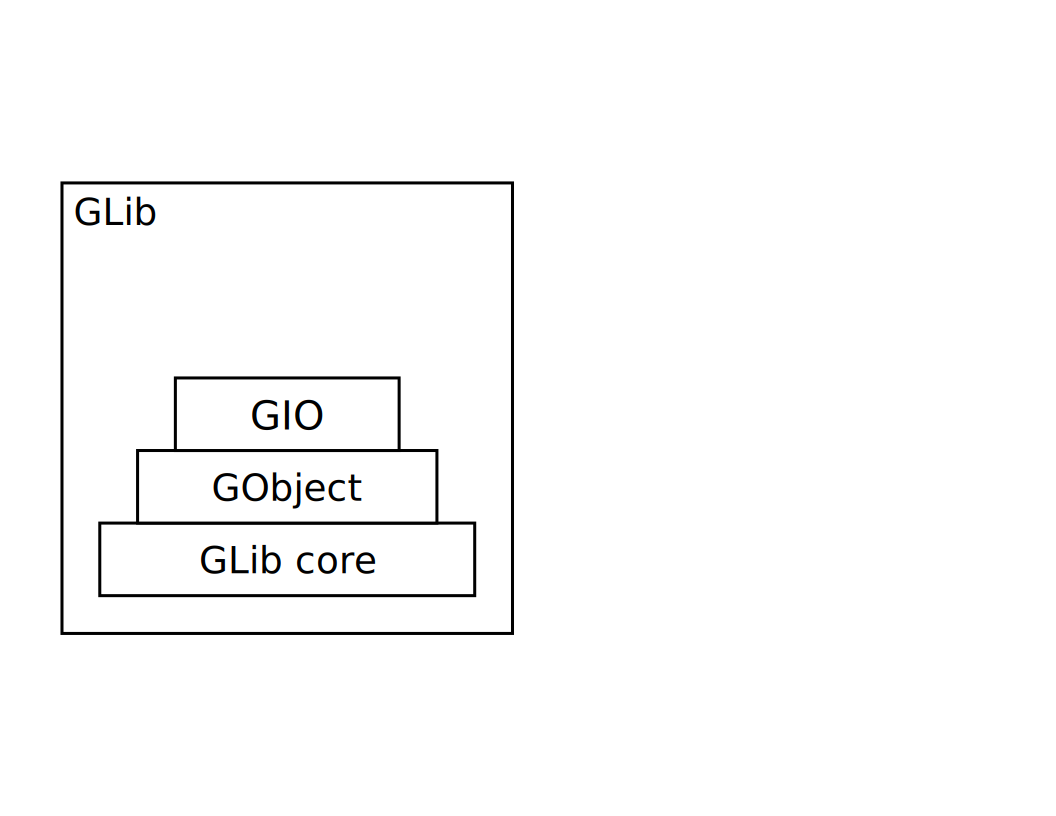
\includegraphics[width=4cm]{assets/img/diag/glib-struct-001.pdf}
    \caption{Estructura de la biblioteca GLib.}
    \label{fig-glib-struct-001}
\end{figure}

Las bibliotecas GLib se pueden utilizar para escribir servicios del sistema operativo, bibliotecas, utilidades de línea de comandos y demás. GLib ofrece API de mayor nivel que el estándar POSIX; por lo tanto, es más cómodo escribir un programa en C con GLib.

GTK es un conjunto de herramientas de widgets basado en GLib que se puede utilizar para desarrollar aplicaciones con una interfaz gráfica de usuario (GUI). Un ``widget'' es un elemento de la GUI, por ejemplo, un botón, un texto, un menú, etc. Y hay algunos tipos especiales de widgets que se denominan ``containers'', que pueden contener otros widgets, para ensamblar los elementos en una ventana. GTK proporciona una amplia gama de widgets y contenedores.

La primera versión de GTK, o GIMP Tool Kit\footnote{El nombre ``The GIMP Tool Kit'' ahora rara vez se usa, hoy se conoce más comúnmente como GTK para abreviar.}, fue escrita principalmente por Peter~Mattis en 1996 para GIMP (Programa de manipulación de imágenes GNU), pero se ha convertido rápidamente en una biblioteca de uso general. Una vez el proyecto se movió fuera del árbol de fuentes de GIMP para distinguir entre la versión original y una nueva versión que agregó características orientadas a objetos se agrego al nombre un ``+'' denominándose la biblioteca como GTK+ (actualmente este nombre esta en desuso y se conoce simplemente como GTK). GLib comenzó como parte de GTK, pero ahora es una biblioteca independiente.

Las API GLib y GTK están documentadas con GTK-Doc. Los comentarios especiales están escritos en el código fuente y GTK-Doc extrae esos comentarios para generar páginas HTML.

Aunque GLib y GTK están escritos en C, los enlaces de lenguaje están disponibles para JavaScript, Python, Perl y muchos otros lenguajes de programación. Al principio, se crearon enlaces manuales, que debían actualizarse cada vez que cambiaba la API de la biblioteca. Hoy en día, los enlaces de lenguaje son genéricos y, por lo tanto, se actualizan automáticamente cuando, por ejemplo, se agregan nuevas funciones, esto es gracias a GObject Introspection . Se agregan anotaciones especiales a los comentarios de GTK-Doc, para exponer más información de la que puede proporcionar la sintaxis de C, por ejemplo, sobre la transferencia de propiedad de contenido asignado dinámicamente\footnote{Por ejemplo, si necesita liberar el valor de retorno.}. Además, las anotaciones también son útiles para el programador en C porque es una forma buena y concisa de documentar ciertos aspectos recurrentes de la API.

En el momento de escribir este artículo, hay nuevas versiones estables de GLib y GTK cada seis meses, alrededor de marzo y septiembre. Un número de versión tiene la forma ``\texttt{major.minor.micro}'', donde ``\texttt{minor}'' designa ciclos estables si es par y ciclos de desarrollo (versiones inestables) si es impar.  Por ejemplo, las versiones 4.4.* son estables, pero las versiones 4.5.* son inestables. Una nueva versión ``\texttt{micro}'' estable (por ejemplo, 4.4.0 $\rightarrow$ 4.4.1) no agrega nuevas funciones, solo actualizaciones de traducción, corrección de errores y mejoras de rendimiento. Para una biblioteca, un nuevo número de versión ``\texttt{major}'' generalmente significa que ha habido una ruptura de la API, pero afortunadamente las versiones principales anteriores se pueden instalar en paralelo con la nueva versión. Durante un ciclo de desarrollo (por ejemplo, 4.5), no hay garantías de estabilidad en la API para \emph{nuevas} funciones; pero al ser uno de los primeros en adoptarlo, sus comentarios son útiles para descubrir más rápidamente fallas y errores de diseño.

GLib y GTK son parte del Proyecto GNU, cuyo objetivo general es desarrollar un sistema operativo libre (llamado GNU) más aplicaciones que lo acompañen. GNU significa ``GNU's Not Unix'', una forma divertida de decir que el sistema operativo GNU es compatible con Unix. Puede obtener más información sobre GNU en \url{https://www.gnu.org}.

El sitio web de GLib/GTK es: \url{http://www.gtk.org}

\section{El escritorio GNOME}

Un proyecto importante para GLib y GTK es GNOME. GNOME, que también forma parte de GNU, es un entorno de escritorio libre iniciado en 1997 por Miguel~de~Icaza y Federico~Mena-Quintero. GNOME hace un uso extensivo de GTK, y este último ahora es desarrollado principalmente por desarrolladores de GNOME.

``GNOME'' es en realidad un acrónimo: GNU Network Object Model Environment\footnote{Como con GTK, el nombre completo de GNOME rara vez se usa y no refleja la realidad actual.}. Originalmente, el proyecto tenía la intención de crear un marco para objetos de aplicación, similar a las tecnologías OLE y COM de Microsoft. Sin embargo, el alcance del proyecto se expandió rápidamente; quedó claro se requería un trabajo preliminar sustancial antes de que la parte del nombre de ``network object'' pudiera convertirse en realidad. Las versiones antiguas de GNOME incluían una arquitectura de incrustación de objetos llamada Bonobo, y GNOME 1.0 incluía un ORB CORBA rápido y ligero llamado ORBit. Bonobo ha sido reemplazado por D-Bus un sistema de comunicación entre procesos.

GNOME tiene dos caras importantes. Desde la perspectiva del usuario, es un entorno de escritorio integrado y una suite de aplicaciones. Desde la perspectiva del programador, es un marco de desarrollo de aplicaciones (compuesto por numerosas bibliotecas útiles que se basan en GLib y GTK). Las aplicaciones escritas con las bibliotecas de GNOME funcionan bien incluso si el usuario no está ejecutando el entorno de escritorio, pero se integran bien con el escritorio de GNOME si está disponible.

El entorno de escritorio incluye un ``shell'' para cambiar de tareas y ejecutar programas, un ``centro de control'' para la configuración, muchas aplicaciones como un administrador de archivos, un navegador web, un reproductor de películas, etc. Estos programas ocultan la línea de comandos tradicional de Unix detrás de una interfaz gráfica fácil de usar.

El marco de desarrollo de GNOME permite escribir aplicaciones interoperables, coherentes y fáciles de usar. Los diseñadores de sistemas de ventanas como X11 o Wayland tomaron la decisión deliberada de no imponer ninguna política de interfaz de usuario a los desarrolladores; GNOME agrega una ``capa de política'', creando una apariencia coherente. Las aplicaciones GNOME terminadas funcionan bien con el escritorio GNOME, pero también se pueden usar de forma ``independiente'' -- los usuarios solo necesitan instalar las bibliotecas compartidas de GNOME. Una aplicación GNOME no está vinculada a un sistema de ventanas específico, GTK proporciona backends para X Window System, Wayland, Mac OS X, Windows e incluso para un navegador web.

Los componentes de GNOME deben instalarse con las mismas versiones, junto con la versión de GTK y GLib lanzada al mismo tiempo; por ejemplo, es una mala idea ejecutar un demonio GNOME en la versión 41 con el centro de control en la versión 40. En el momento de escribir este libro, las últimas versiones estables son: GLib~2.70, GTK~4.4 y GNOME~41, todas lanzadas en el segundo semestre de 2021. 

Más información sobre GNOME: \url{https://www.gnome.org/}

\section{Prerrequisitos}

Este libro asume que ya tiene algo de práctica en programación. A continuación, se muestra una lista de requisitos previos recomendados, con referencias de libros.

\begin{itemize}
    \item Este texto supone que ya conoce el lenguaje C. El libro de referencia es \emph{The C Programming Language}, de Brian Kernighan y Dennis Ritchie \cite{k-r-book}.
    
    \item La programación orientada a objetos (OOP) también es necesaria para aprender GObject. Debe estar familiarizado con conceptos como herencia, una interfaz, un método virtual o polimorfismo. Un buen libro, con más de sesenta pautas, es \emph{Heurística de diseño orientado a objetos}, de Arthur~Riel \cite{oop-book}.
    
    \item Es útil haber leído un libro sobre estructuras de datos y algoritmos, pero puede aprenderlo en paralelo. Un libro recomendado es \emph{The Algorithm Design Manual}, de Steven~Skiena \cite{algo-book}.
    
    \item Si desea desarrollar su software en un sistema similar a Unix, otro requisito previo es saber cómo funciona Unix y estar familiarizado con la línea de comandos, un poco de scripts de shell y cómo escribir un Makefile. Un posible libro es \emph{UNIX for the Impatient}, de Paul~Abrahams \cite{unix-impatient}.
    
    \item No es estrictamente necesario, pero se recomienda encarecidamente utilizar un sistema de control de versiones como Git. Un buen libro es \emph{Pro Git}, de Scott~Chacon \cite{pro-git}.
\end{itemize}

\section{¿Por qué y cuándo se usa el lenguaje C?}

Las bibliotecas GLib y GTK pueden ser utilizadas por otros lenguajes de programación además de C. Gracias a GObject Introspection, los enlaces automáticos están disponibles para una gran variedad de lenguajes, de manera que puedan ser usadas todas las bibliotecas basadas en GObject por estos. Los enlaces oficiales de GNOME están disponibles para los siguientes lenguajes \footnote{Aunque existen enlaces a más lenguajes, los expresados en la tabla son los más activos es sus repositorios y con una mayor comunidad.}:

\begin{table}[H]
    \centering
    \begin{tabular}{|l|l|l|l|}
    \hline
    \multicolumn{1}{|c|}{\textbf{Lenguaje}} & \multicolumn{1}{c|}{\textbf{v3}} & \multicolumn{1}{c|}{\textbf{v4}} & \multicolumn{1}{c|}{\textbf{Enlace}} \\ \hline
    C++        & \faIcon[regular]{check-square} & \faIcon[regular]{check-square} & \url{https://www.gtkmm.org/}            \\ \hline
    JavaScript & \faIcon[regular]{check-square} & \faIcon[regular]{check-square} & \url{https://gjs.guide/}                \\ \hline
    Python     & \faIcon[regular]{check-square} & \faIcon[regular]{check-square} & \url{https://pygobject.readthedocs.io/} \\ \hline
    Rust       & \faIcon[regular]{check-square} & \faIcon[regular]{check-square} & \url{https://gtk-rs.org/}               \\ \hline
    Vala       & \faIcon[regular]{check-square} & \faIcon[regular]{check-square} & \url{https://valadoc.org/}              \\ \hline
    \end{tabular}
\end{table}

Una buena alternativa a C es Vala, el cual es un lenguaje de programación que integra las peculiaridades de GObject directamente en su sintaxis similar a C\#. De manera que todo el código hecho en Vala es traducido a código en C, el cual hace uso de GObject directamente, esto puede resultar útil si desea código cercano a C pero haciendo uso de un lenguaje más moderno\footnote{Tenga en cuenta que el lenguaje Vala podría considerarse un lenguaje de nicho, teniendo una comunidad pequeña si es comparado con lenguajes más populares.}.

Otra alternativa importante a considerar si desea trabajar con GLib/GTK es el lenguaje Rust, un lenguaje moderno que genera programas eficientes en memoria, gracias a un verificador de prestamos que validan las referencias, por lo cual no necesita de un recolector de basura como otros lenguajes de programación para asegurar la seguridad de la memoria.

Más allá de los enlaces oficiales de GNOME; GLib y GTK se pueden usar en más de una docena de lenguajes de programación, con un nivel de soporte variable. Entonces, \emph{¿por qué y cuándo elegir el lenguaje C?}.

Por ejemplo, para escribir un demonio en un sistema tipo Unix, C es el lenguaje \emph{predeterminado}. Pero es menos obvio que lenguaje usar para una aplicación. Para responder a la pregunta, veamos primero cómo estructurar el código base de una aplicación.

% Adaptado de una pregunta de preguntas frecuentes en GGAD.
\subsection{Separación de backend del frontend}
\label{intro-backend-frontend-separation}
Una buena práctica es separar la interfaz gráfica de usuario del resto de la aplicación. Por diversas razones, la interfaz gráfica de una aplicación tiende a ser una pieza de software excepcionalmente volátil y en constante cambio. Es el foco de la mayoría de las solicitudes de cambio de los usuarios. Es difícil planificar y ejecutar bien la primera vez; a menudo descubrirá que algún aspecto es desagradable de usar solo después de haberlo escrito. A veces es deseable tener varias interfaces de usuario diferentes, por ejemplo, una versión de línea de comandos o una interfaz basada en web.

En términos prácticos, esto significa que cualquier aplicación grande debe tener una separación radical entre sus diversos \emph{frontends} o interfaces y el \emph{backend}. El backend debe contener todas las ``partes complejas'': sus algoritmos y estructuras de datos, el trabajo real realizado por la aplicación. Piense en ello como un ``modelo'' abstracto que se muestra y manipula el usuario.

Cada interfaz debe ser una ``vista'' y un ``controlador''. Como una ``vista'', la interfaz debe anotar cualquier cambio en el backend y cambiar la pantalla en consecuencia. Como un ``controlador'', la interfaz debe permitir al usuario transmitir solicitudes de cambio al backend (define cómo las manipulaciones de la interfaz se traducen en cambios en el modelo).

Hay muchas formas de disciplinarse para mantener su aplicación separada. Un par de ideas útiles:

\begin{itemize}
    \item Escriba el backend como una biblioteca. Al principio, la biblioteca puede ser interna a la aplicación y estar vinculada estáticamente, sin garantías de estabilidad API/ABI. Cuando el proyecto crezca, y si el código es útil para otros programas, puede convertir fácilmente su backend en una biblioteca compartida.
    \item Escriba al menos dos interfaces desde el principio; uno o ambos pueden ser prototipos feos, solo desea tener una idea de cómo estructurar el backend. Recuerde, las interfaces deben ser fáciles; el backend tiene las partes difíciles.
\end{itemize}

El lenguaje C es una buena opción para la parte de backend de una aplicación. Al utilizar GObject y GObject Introspection, su biblioteca estará disponible para otros proyectos escritos en varios lenguajes de programación. Por otro lado, una biblioteca de Python o JavaScript no se puede utilizar en otros lenguajes. Para las interfaces, un idioma de nivel superior puede ser más conveniente, dependiendo de los idiomas con los que ya domine.

\subsection{Otros aspectos a tener en cuenta}
Si tiene dudas sobre el lenguaje a elegir, aquí hay otros aspectos a tener en cuenta. Tenga en cuenta que este texto está un poco sesgado ya que se eligió el lenguaje C.

C es un lenguaje de tipo estático: los tipos de variables y los prototipos de funciones en un programa se conocen en el momento de la compilación. El compilador descubre muchos errores triviales, como un error tipográfico en el nombre de una función. El compilador también es de gran ayuda cuando se hacen refactorizaciones de código, lo cual es esencial para el mantenimiento a largo plazo de un programa. Por ejemplo, cuando divide una clase en dos, si el código que usa la clase inicial no se actualiza correctamente, el compilador se lo informará amablemente\footnote{Bueno, \emph{amablemente} quizás no sea la mejor descripción, arrojar un montón de errores está más cerca de la realidad.}. Con el desarrollo basado en pruebas (TDD), y escribiendo pruebas unitarias para \emph{todo}, también es factible escribir una enorme base de código en un lenguaje de tipo dinámico como Python. Con una muy buena cobertura de código, las pruebas unitarias también detectarán errores al refactorizar el código. Pero las pruebas unitarias pueden ser mucho más lentas de ejecutar que compilar el código, ya que también prueba el comportamiento del programa. Por lo tanto, puede que no sea conveniente ejecutar todas las pruebas unitarias al realizar refactorizaciones de código. ¡Por supuesto, escribir pruebas unitarias también es una buena práctica para una base de código C! Sin embargo, para la parte GUI del código, escribir pruebas unitarias a menudo no es una tarea de alta prioridad si la aplicación está bien probada por sus desarrolladores.

C es un lenguaje escrito explícitamente: los tipos de variables son visibles en el código. Es una forma de auto-documentar el código; por lo general, no es necesario agregar comentarios para explicar qué contienen las variables. Conocer el tipo de variable es importante para comprender el código, saber qué representa la variable y qué funciones se pueden llamar sobre ella. En un asunto relacionado, el objeto \emph{self} se pasa explícitamente como un argumento de función. Por lo tanto, cuando se accede a un atributo a través del puntero \emph{self}, se sabe de dónde procede el atributo. Algunos lenguajes orientados a objetos tienen \emph{esta} palabra clave para ese propósito, pero a veces es opcional como en C ++ o Java. En este último caso, una función útil del editor de texto es resaltar atributos de manera diferente, por lo que incluso cuando no se usa \emph{esta} palabra clave, usted sabe que es un atributo y no una variable local. Con el objeto \emph{self} pasado como argumento, no hay posibles confusiones.

El lenguaje C tiene una \emph{cadena de herramientas} muy buena: compiladores estables (GCC, Clang,...), Editores de texto (Vim, Emacs,...), Depuradores (GDB, Valgrind,...), Herramientas de análisis estático, ...

Para algunos programas, un recolector de basura no es apropiado porque pausa el programa regularmente para liberar la memoria no utilizada. Para secciones de código críticas, como animaciones en tiempo real, no es conveniente pausar el programa (un recolector de basura a veces puede ejecutarse durante varios segundos). En este caso, la gestión manual de la memoria como en C es una solución.

Menos importante, pero útil; la verbosidad de C en combinación con las convenciones GLib/GTK tiene una ventaja: el código se puede buscar fácilmente con un comando como \shellcmd{grep}. Por ejemplo, la función \lstinline{gtk_widget_show()} contiene el espacio de nombres (\lstinline{gtk}), la clase (\lstinline{widget}) y el método (\lstinline{show}). Con un lenguaje orientado a objetos, la sintaxis es generalmente \lstinline[language=C++]{object.show()}. Si se busca ``show'' en el código, probablemente habrá más falsos positivos, por lo que se necesita una herramienta más inteligente. Otra ventaja es que conocer el espacio de nombres y la clase de un método puede ser útil al leer el código, es otra forma de auto-documentación.


Más importante aún, la documentación de la API GLib/GTK está escrita principalmente para el lenguaje C. No es conveniente leer la documentación de C mientras se programa en otro idioma. Algunas herramientas están actualmente en desarrollo para generar la documentación de la API para otros lenguajes de destino, por lo que es de esperar que en el futuro ya no sea un problema.

GLib/GTK están escritos en C. Entonces, cuando se programa en C, no hay capa adicional. Una capa adicional es potencialmente una fuente de errores adicionales y cargas de mantenimiento. Además, usar el lenguaje C probablemente sea mejor para propósitos pedagógicos. Un lenguaje de nivel superior puede ocultar algunos detalles sobre GLib/GTK. Por lo tanto, el código es más corto, pero cuando tiene un problema, debe comprender no solo cómo funciona la función de la biblioteca, sino también cómo funciona el enlace del idioma.

Dicho esto, si:

\begin{enumerate}
    \item No se siente cómodo en C.
    \item Ya domina un lenguaje de nivel superior con compatibilidad con GObject Introspection.
    \item Planea escribir solo una pequeña aplicación o complemento.
\end{enumerate}

Elegir un lenguaje de nivel superior tiene mucho sentido.

\section{Ruta de aprendizaje}
\label{intro-learning-path}
% PARA HACER cuando el libro esté terminado, cambie el nombre de esta sección a "Estructura del libro"

Normalmente, esta sección debería llamarse ``Estructura del libro'', pero como puede ver, el libro está lejos de estar terminado, por lo que la sección se llama ``Ruta de aprendizaje''.

El camino de aprendizaje lógico es:
\begin{enumerate}
    \item Los fundamentos del núcleo GLib;
    \item Programación orientada a objetos en C y los conceptos básicos de GObject;
    \item GTK y GIO en paralelo.
\end{enumerate}

Dado que GTK se basa en GLib y GObject, es mejor comprender primero los conceptos básicos de esas dos bibliotecas. Algunos tutoriales se sumergen directamente en GTK, por lo que después de un corto período de tiempo puede mostrar una ventana con texto y tres botones; es divertido, pero conocer GLib y GObject no es un lujo si quiere comprender lo que está haciendo, y una aplicación GTK realista utiliza ampliamente las bibliotecas GLib. GTK y GIO se pueden aprender en paralelo --- una vez que comience a usar GTK, verá que algunas partes que no son GUI están basadas en GIO.

Así que este libro comienza con la biblioteca principal GLib (parte~\ref{glib} p.~\pageref{glib}), luego presenta la Programación Orientada a Objetos en C (parte~\ref{oop} p.~\pageref{oop}) seguida de un capítulo de Lecturas Adicionales (p.~\pageref{further-reading})

\section{El entorno de desarrollo}
\label{intro-dev-environment}

Esta sección describe el entorno de desarrollo que se usa normalmente al programar con GLib y GTK en un sistema Unix.

En una distribución GNU/Linux, a menudo se puede instalar un solo paquete o grupo para obtener un entorno de desarrollo C completo, que incluye, entre otros:
\begin{itemize}
    \item Un compilador compatible con C89, GCC por ejemplo;
    \item El depurador GNU GDB;
    \item GNU Make;
    \item Las Autotools (Autoconf, Automake y Libtool);
    \item Las páginas del manual de: El kernel de Linux y glibc \footnote{No confunda la biblioteca GNU C (glibc) con GLib. El primero es de nivel inferior.}.
\end{itemize}

Para utilizar GLib y GTK como desarrollador, existen varias soluciones:
\begin{itemize}
    \item Los encabezados y la documentación se pueden instalar con el administrador de paquetes. El nombre de los paquetes suele terminar con uno de los siguientes sufijos: \texttt{-devel}, \texttt{-dev} o \texttt{-doc}. Por ejemplo \texttt{glib2-devel} y \texttt{glib2-doc} en Fedora.
    \item Las últimas versiones de GLib y GTK se pueden instalar con Jhbuild:\\
    \url{https://wiki.gnome.org/Projects/Jhbuild}
\end{itemize}

Para leer la documentación de la API de GLib y GTK, Devhelp es una aplicación útil, si ha instalado el paquete -dev o -doc. Para el editor de texto o IDE, hay muchas opciones (y una fuente de muchos trolls): Vim, Emacs, gedit, Anjuta, MonoDevelop/Xamarin Studio, Geany,… Un prometedor IDE especializado para GNOME es Builder, actualmente en desarrollo. Para crear una GUI con GTK, puede escribir directamente el código para hacerlo o puede usar Glade para diseñar la GUI gráficamente. Finalmente, GTK-Doc se usa para escribir documentación de API y agregar las anotaciones de GObject Introspection.

Cuando utilice GLib o GTK, preste atención a no utilizar API obsoletas para el código recién escrito. Asegúrese de leer la documentación más reciente. También están disponibles en línea en:\\

\url{https://developer.gnome.org/}

\part{GLib, la biblioteca principal\label{glib}}

\chapter{GLib, la biblioteca principal}

GLib es la biblioteca central de bajo nivel que forma la base para proyectos como GTK y GNOME. Proporciona estructuras de datos, funciones de utilidad, envoltorios de portabilidad y otras funciones esenciales, como un bucle de eventos e hilos. GLib está disponible en la mayoría de los sistemas similares a Unix y Windows.

Este capítulo cubre algunas de las funciones más utilizadas. GLib es simple y los conceptos son familiares; así que nos moveremos rápidamente. Para obtener una cobertura más completa de GLib, consulte la última documentación de la API que viene con la biblioteca (para el entorno de desarrollo, consulte la sección~\ref{intro-dev-env} en la p.~\pageref{intro-dev-env}). Por cierto: si tiene preguntas muy específicas sobre la implementación, no tema mirar el código fuente. Normalmente, la documentación contiene suficiente información, pero si encuentra un detalle faltante, por favor presente un error (por supuesto, lo mejor sería con un parche proporcionado).

Las diversas instalaciones de GLib están destinadas a tener una interfaz coherente; el estilo de codificación está orientado a semiobjetos, y los identificadores tienen el prefijo ``g'' para crear una especie de espacio de nombres.

GLib tiene algunos encabezados de nivel superior:
\begin{itemize}
    \item \path{glib.h}, el encabezado principal;
    \item \path{gmodule.h} para carga dinámica de módulos;
    \item \path{glib-unix.h} para API específicas de Unix;
    \item \path{glib/gi18n.h} y \path{glib/gi18n-lib.h} para la internacionalización;
    \item \path{glib/gprintf.h} y \path{glib/gstdio.h} para evitar tirar de todo stdio.
\end{itemize}

\bigskip
Nota: en lugar de reinventar la rueda, este capítulo se basa en gran medida en el capítulo correspondiente del libro \emph{GTK+/Gnome Application Development} de Havoc Pennington, con licencia de Open Publication License (consulte la sección~\ref{intro-license} p.~\pageref{intro-license}). GLib tiene una API muy estable. A pesar de que el libro de Havoc Pennington fue escrito en 1999 (para GLib 1.2), solo se requirieron algunas actualizaciones para adaptarse a las últimas versiones de GLib (versión~2.70 en el momento de escribir este artículo)

\section{Lo esencial}

GLib proporciona sustitutos para muchas construcciones de lenguaje C estándar y de uso común. Esta sección describe las definiciones de tipos fundamentales, macros, rutinas de asignación de memoria y funciones de utilidad de cadena de GLib.

\subsection{Definiciones de tipo}

En lugar de utilizar los tipos estándar de C (\lstinline{int}, \lstinline{long}, etc.), GLib define los suyos propios. Estos sirven para una variedad de propósitos. Por ejemplo, se garantiza que \lstinline{gint32} tiene 32 bits de ancho, algo que ningún tipo C89 estándar puede garantizar. \lstinline{guint} es simplemente más fácil de escribir que \lstinline{unsigned}. Algunos de los typedefs existen solo por coherencia; por ejemplo, \lstinline{gchar} siempre es equivalente al \lstinline{char} estándar.

Los tipos primitivos más importantes definidos por GLib:
\begin{itemize}
    \item \lstinline{gint8}, \lstinline{guint8}, \lstinline{gint16}, \lstinline{guint16}, \lstinline{gint32}, \lstinline{guint32}, \lstinline{gint64}, \lstinline{guint64} --- le dará números enteros de un tamaño garantizado. (Si no es obvio, los tipos \lstinline{guint} son unsigned, los tipos de gint son signed).
    
    \item \lstinline{gboolean} es útil para hacer su código más legible, ya que C89 no tiene un tipo \lstinline{bool}.
    
    \item \lstinline{gchar}, \lstinline{gshort}, \lstinline{glong}, \lstinline{gint}, \lstinline{gfloat}, \lstinline{gdouble} son puramente cosméticos.
    
    \item \lstinline{gpointer} puede ser más conveniente de escribir que \lstinline{void *}. \lstinline{gconstpointer} le da \lstinline{const void *}. (\lstinline{const gpointer} no hará lo que normalmente quiere; dedique un tiempo a leer un buen libro sobre C si no ve por qué).
    
    \item \lstinline{gsize} es un tipo entero sin signo que puede contener el resultado del operador \lstinline{sizeof}.
\end{itemize}

\subsection{Macros de uso frecuente}

GLib define una serie de macros familiares que se utilizan en muchos programas C, que se muestran en el Listado~\ref{glib-simplemacros}. Todos estos deben ser autoexplicativos. \lstinline{MIN()}/\lstinline{MAX()} devuelven el menor o mayor de sus argumentos. \lstinline{ABS()} devuelve el valor absoluto de su argumento. \lstinline{CLAMP(x, low, high)} significa \lstinline{x}, a menos que \lstinline{x} esté fuera del rango [\lstinline{low},~\lstinline{high}]; si \lstinline{x} está por debajo del rango, se devuelve \lstinline{low}; si \lstinline{x} está por encima del rango, se devuelve \lstinline{high}. Además de las macros que se muestran en el Listado~\ref{glib-simplemacros}, \lstinline{TRUE}/\lstinline{FALSE}/\lstinline{NULL} se definen como los habituales \lstinline{1}/\lstinline{0}/\lstinline{((void *)0)}.

\begin{lstlisting}[style=GLib/GTK, caption={Macros C familiares}, label=glib-simplemacros]
#include <glib.h>

MAX (a, b);
MIN (a, b);
ABS (x);
CLAMP (x, low, high);
\end{lstlisting}

También hay muchas macros exclusivas de GLib, como las conversiones portátiles \lstinline{gpointer}-to-\lstinline{gint} y \lstinline{gpointer}-to-\lstinline{guint} que se muestran en el Listado ~\ref{glib-pointerint}.

\begin{lstlisting}[style=GLib/GTK, caption={Macros para almacenar enteros en punteros}, label=glib-pointerint]
#include <glib.h>

GINT_TO_POINTER (p);
GPOINTER_TO_INT (p);
GUINT_TO_POINTER (p);
GPOINTER_TO_UINT (p);
\end{lstlisting}

La mayoría de las estructuras de datos de GLib están diseñadas para almacenar un \lstinline{gpointer}. Si desea almacenar punteros a objetos asignados dinámicamente, esto es lo correcto. Sin embargo, a veces desea almacenar una lista simple de números enteros sin tener que asignarlos dinámicamente. Aunque el estándar C no lo garantiza estrictamente, es posible almacenar un \lstinline{gint} o \lstinline{guint} en una variable \lstinline{gpointer} en la amplia gama de plataformas a las que GLib ha sido portado; en algunos casos, se requiere un yeso intermedio. Las macros en Listado~\ref{glib-pointerint} abstraen la presencia del elenco.

He aquí un ejemplo:
\begin{lstlisting}[style=GLib/GTK]
gint my_int;
gpointer my_pointer;

my_int = 5;
my_pointer = GINT_TO_POINTER (my_int);
printf ("Estamos almacenando %d\n", GPOINTER_TO_INT (my_pointer));
\end{lstlisting}

Pero tenga cuidado; estas macros le permiten almacenar un entero en un puntero, pero almacenar un puntero en un entero \emph{no} funcionará. Para hacerlo de forma portátil, debe almacenar el puntero en un \lstinline{long}. (Sin embargo, sin duda es una mala idea hacerlo).

\subsection{Macros de depuración}
\label{glib-debugging-macros}

GLib tiene un buen conjunto de macros que puede usar para hacer cumplir invariantes y condiciones previas en su código. GTK los usa generosamente, una de las razones por las que es tan estable y fácil de usar. Todos desaparecen cuando define \lstinline{G_DISABLE_CHECKS} o \lstinline{G_DISABLE_ASSERT}, por lo que no hay penalización de rendimiento en el código de producción. Usarlos generosamente es una muy, muy buena idea. Encontrará errores mucho más rápido si lo hace. Incluso puede agregar afirmaciones y verificaciones cada vez que encuentre un error para asegurarse de que el error no vuelva a aparecer en versiones futuras; esto complementa un conjunto de regresión. Las comprobaciones son especialmente útiles cuando el código que está escribiendo será utilizado como caja negra por otros programadores; los usuarios sabrán inmediatamente cuándo y cómo han hecho un mal uso de su código.

Por supuesto, debe tener mucho cuidado de asegurarse de que su código no dependa sutilmente de declaraciones de solo depuración para funcionar correctamente. Las declaraciones que desaparecerán en el código de producción \emph{nunca} deberían tener efectos secundarios.

\begin{lstlisting}[style=GLib/GTK, caption={Comprobaciones de condiciones previas}, label=glib-precondition]
#include <glib.h>

g_return_if_fail (condition);
g_return_val_if_fail (condition, return_value);
\end{lstlisting}

% PARA HACER agregar la referencia del capítulo de gobject cuando el capítulo esté escrito
El Listado~\ref{glib-precondition} muestra las verificaciones de condiciones previas de GLib. \lstinline{g_return_if_fail()} imprime una advertencia y regresa inmediatamente de la función actual si \lstinline{condition} es \lstinline{FALSE}. \lstinline{g_return_val_if_fail()} es similar pero le permite devolver algún \lstinline{return_value}. Estos macros son increíblemente útiles, si las usa libremente, especialmente en combinación con la verificación de tipo en tiempo de ejecución de GObject, %(ver capitulo~\ref{oop-gobject})
reducirá a la mitad el tiempo que dedica a buscar punteros incorrectos y errores tipográficos.

Usar estas funciones es simple; aquí hay un ejemplo de la implementación de la tabla hash GLib:
\begin{lstlisting}[style=GLib/GTK]
void
g_hash_table_foreach (GHashTable *hash_table,
                      GHFunc      func,
                      gpointer    user_data)
{
  gint i;

  g_return_if_fail (hash_table != NULL);
  g_return_if_fail (func != NULL);

  for (i = 0; i < hash_table->size; i++)
    {
      guint node_hash = hash_table->hashes[i];
      gpointer node_key = hash_table->keys[i];
      gpointer node_value = hash_table->values[i];

      if (HASH_IS_REAL (node_hash))
        (* func) (node_key, node_value, user_data);
    }
}
\end{lstlisting}

Sin las comprobaciones, pasar \lstinline{NULL} como parámetro a esta función resultaría en una misteriosa falla de segmentación. La persona que usa la biblioteca tendría que averiguar dónde ocurrió el error con un depurador y tal vez incluso indagar en el código GLib para ver qué estaba mal. Con las comprobaciones, obtendrán un mensaje de error que les indicará que los argumentos \lstinline{NULL} no están permitidos.

\begin{lstlisting}[style=GLib/GTK, caption={Aserciones}, label=glib-assertions]
#include <glib.h>

g_assert (condition);
g_assert_not_reached ();
\end{lstlisting}

GLib también tiene macros de aserción más tradicionales, que se muestran en el Listado~\ref{glib-assertions}. \lstinline{g_assert()} es básicamente idéntico a \lstinline{assert()}, pero responde a \lstinline{G_DISABLE_ASSERT} y se comporta consistentemente en todas las plataformas. También se proporciona \lstinline{g_assert_not_reached()}; esta es una aserción que siempre falla. Las aserciones llaman a \lstinline{abort()} para salir del programa y (si su entorno lo admite) descargan un archivo central con fines de depuración.

Las aserciones fatales deben usarse para verificar la \emph{consistencia interna} de una función o biblioteca, mientras que \lstinline{g_return_if_fail()} está destinado a garantizar que se pasen valores cuerdos a las interfaces públicas de un módulo de programa. Es decir, si una aserción falla, normalmente busca un error en el módulo que contiene la aserción; Si falla una comprobación de \lstinline{g_return_if_fail()}, normalmente busca el error en el código que invoca el módulo.

Este código del módulo de cálculos calendáricos de GLib muestra la diferencia:
\begin{lstlisting}[style=GLib/GTK]
GDate *
g_date_new_dmy (GDateDay   day,
                GDateMonth month,
                GDateYear  year)
{
  GDate *date;
  g_return_val_if_fail (g_date_valid_dmy (day, month, year), NULL);

  date = g_new (GDate, 1);

  date->julian = FALSE;
  date->dmy = TRUE;

  date->month = month;
  date->day = day;
  date->year = year;

  g_assert (g_date_valid (date));

  return date;
}
\end{lstlisting}

La verificación de condiciones previas al principio asegura que el usuario pasa en valores razonables para el día, mes y año; la aserción al final asegura que GLib construyó un objeto correctamente, dados valores adecuados.

\lstinline{g_assert_not_reached()} debe usarse para marcar situaciones ``imposibles''; un uso común es detectar declaraciones de cambio que no manejan todos los valores posibles de una enumeración:

\begin{lstlisting}[style=GLib/GTK]
switch (value)
  {
  case FOO_ONE:
    break;

  case FOO_TWO:
    break;

  default:
    g_assert_not_reached ();
  }
\end{lstlisting}

Todas las macros de depuración imprimen una advertencia utilizando la función \lstinline{g_log()} de GLib, lo que significa que la advertencia incluye el nombre de la aplicación o biblioteca de origen y, opcionalmente, puede instalar una rutina de impresión de advertencias de reemplazo. Por ejemplo, puede enviar todas las advertencias a un cuadro de diálogo o archivo de registro en lugar de imprimirlas en la consola.

\subsection{Memoria}

GLib envuelve el estándar \lstinline{malloc()} y \lstinline{free()} con sus propias variantes \lstinline{g_}, \lstinline{g_malloc()} y \lstinline{g_free()}, que se muestran en el Listado~\ref{glib-malloc-free}.
Estos son agradables de varias maneras pequeñas:

\begin{itemize}
    \item \lstinline{g_malloc()} siempre devuelve un \lstinline{gpointer}, nunca un \lstinline{char *}, por lo que no es necesario emitir el valor de retorno \footnote{Antes del estándar ANSI/ISO C, el tipo de puntero genérico \lstinline{void *} no existía y \lstinline{malloc()} devolvía un valor \lstinline{char *}. Actualmente, \lstinline{malloc()} devuelve un tipo \lstinline{void *} ---~que es lo mismo que \lstinline{gpointer}~--- y \lstinline{void *} permite conversiones de puntero implícitas en C. Lanzando el valor de retorno de \lstinline{malloc()} es necesario si: el desarrollador quiere admitir compiladores antiguos; o si el desarrollador piensa que una conversión explícita aclara el código; o si se usa un compilador de C++, porque en C++ se requiere una conversión del tipo \lstinline{void *}.}.
    
    \item \lstinline{g_malloc()} aborta el programa si el \lstinline{malloc()} subyacente falla, por lo que no tiene que buscar un valor devuelto \lstinline{NULL}.
    
    \item \lstinline{g_malloc()} maneja con gracia un \lstinline{size} de \lstinline{0}, devolviendo \lstinline{NULL}.
    
    \item \lstinline{g_free()} ignorará cualquier puntero \lstinline{NULL} que le pase.
\end{itemize}

\begin{lstlisting}[style=GLib/GTK, caption={Asignación de memoria GLib}, label=glib-malloc-free]
#include <glib.h>

gpointer g_malloc (gsize n_bytes);
void g_free (gpointer mem);
gpointer g_realloc (gpointer mem, gsize n_bytes);
gpointer g_memdup (gconstpointer mem, guint n_bytes);
\end{lstlisting}

Es importante hacer coincidir \lstinline{g_malloc()} con \lstinline{g_free()}, \lstinline{malloc()} simple con \lstinline{free()} y (si estás usando C ++) \lstinline[style=GLib/GTK]{new} con \lstinline[style=GLib/GTK]{delete}. De lo contrario, pueden suceder comportamientos no esperados, ya que estos asignadores pueden usar diferentes grupos de memoria (y \lstinline[style=GLib/GTK]{new}/\lstinline[style=GLib/GTK]{delete} llama a constructores y destructores).

Por supuesto, hay un \lstinline{g_realloc()} equivalente a \lstinline{realloc()}. También hay un conveniente \lstinline{g_malloc0()} que llena la memoria asignada con ceros, y \lstinline{g_memdup()} que devuelve una copia de \lstinline{n_bytes} bytes comenzando en \lstinline{mem}. \lstinline{g_realloc()} y \lstinline{g_malloc0()} aceptarán ambos un tamaño de 0, por coherencia con \lstinline{g_malloc()}. Sin embargo, \lstinline{g_memdup()} no lo hará.

% PARA HACER mencionar esto en API doc
Si no es obvio: \lstinline{g_malloc0()} llena la memoria sin procesar con bits no configurados, no el valor 0 para cualquier tipo que pretenda poner allí. De vez en cuando, alguien espera obtener una matriz de números de coma flotante inicializados en 0.0; \emph{no} se garantiza que funcione de forma portátil.

Por último, existen macros de asignación con reconocimiento de tipos, que se muestran en el Listado~\ref{glib-g_new}. El argumento \lstinline{type} para cada uno de estos es el nombre de un tipo, y el argumento \lstinline{count} es el número de bloques de tamaño \lstinline{type} a asignar. Estas macros le ahorran algo de escritura y multiplicación y, por lo tanto, son menos propensas a errores. Se lanzan automáticamente al tipo de puntero de destino, por lo que intentar asignar la memoria asignada al tipo de puntero incorrecto debería activar una advertencia del compilador. (Si tiene las advertencias activadas, ¡como debería hacerlo un programador responsable!)

\begin{lstlisting}[style=GLib/GTK, caption={Macros de asignación}, label=glib-g_new]
#include <glib.h>

g_new (type, count);
g_new0 (type, count);
g_renew (type, mem, count);
\end{lstlisting}

\subsection{Manejo de string}

GLib proporciona una serie de funciones para el manejo de cadenas; algunos son exclusivos de GLib y otros resuelven problemas de portabilidad. Todos interoperan muy bien con las rutinas de asignación de memoria GLib.

Para aquellos interesados en una cadena mejor que \lstinline{gchar *}, también hay un tipo \lstinline{GString}. No se trata en este libro; consulte la documentación de la API para obtener más información.

\begin{lstlisting}[style=GLib/GTK, caption={Envoltorio de portabilidad}, label=glib-strext]
gint g_snprintf (gchar *string, gulong n, gchar const *format, ...);
\end{lstlisting}

El listado~\ref{glib-strext} muestra un sustituto que GLib proporciona para la función \lstinline{snprintf()}. \lstinline{g_snprintf()} envuelve el \lstinline{snprintf()} nativo en las plataformas que lo tienen y proporciona una implementación en las que no lo tienen.

Preste atención a no usar la función \lstinline{sprintf()} que causa fallas, crea agujeros de seguridad y generalmente es maligna. Al usar \lstinline{g_snprintf()} o \lstinline{g_strdup_printf()} relativamente seguros (ver más abajo), puedes despedirte de \lstinline{sprintf()} para siempre.

\begin{lstlisting}[style=GLib/GTK, caption={Asignar cadenas}, label=glib-strdup]
#include <glib.h>

gchar * g_strdup (const gchar *str);
gchar * g_strndup (const gchar *str, gsize n);
gchar * g_strdup_printf (const gchar *format, ...);
gchar * g_strdup_vprintf (const gchar *format, va_list args);
gchar * g_strnfill (gsize length, gchar fill_char);
\end{lstlisting}

El listado~\ref{glib-strdup} muestra la amplia gama de funciones de GLib para asignar cadenas. Como era de esperar, \lstinline{g_strdup()} y \lstinline{g_strndup()} producen una copia asignada de \lstinline{str} o los primeros \lstinline{n} caracteres de \lstinline{str}. Para mantener la coherencia con las funciones de asignación de memoria GLib, devuelven \lstinline{NULL} si se les pasa un puntero \lstinline{NULL}. Las variantes \lstinline{printf()} devuelven una cadena formateada. \lstinline{g_strnfill()} devuelve una cadena de tamaño \lstinline{length} rellena con \lstinline{fill_char}.

\lstinline{g_strdup_printf()} merece una mención especial; es una forma más sencilla de manejar este código común:
\begin{lstlisting}[style=GLib/GTK]
gchar *str = g_malloc (256);
g_snprintf (str, 256, "%d printf-style %s", num, string);
\end{lstlisting}

En su lugar, podría decir esto y evitar tener que averiguar la longitud adecuada del búfer para arrancar:
\begin{lstlisting}[style=GLib/GTK]
gchar *str = g_strdup_printf ("%d printf-style %s", num, string);
\end{lstlisting}

\begin{lstlisting}[style=GLib/GTK, caption={Modificaciones de cadenas in situ}, label=glib-strmanip]
#include <glib.h>

gchar * g_strchug (gchar *string);
gchar * g_strchomp (gchar *string);
gchar * g_strstrip (gchar *string);
\end{lstlisting}

Las funciones del Listado ~\ref{glib-strmanip} modifican una cadena en el lugar: \lstinline{g_strchug()} y \lstinline{g_strchomp()} ``chug'' la cadena (elimina los espacios iniciales), o ``chomp'' (eliminar los espacios finales). Esas dos funciones devuelven la cadena, además de modificarla en el lugar; en algunos casos, puede ser conveniente utilizar el valor de retorno. Hay una macro, \lstinline{g_strstrip()}, que combina ambas funciones para eliminar los espacios iniciales y finales.

\begin{lstlisting}[style=GLib/GTK, caption={Conversiones de cadenas}, label=glib-strformats]
#include <glib.h>

gdouble g_strtod (const gchar *nptr, gchar **endptr);
const gchar * g_strerror (gint errnum);
const gchar * g_strsignal (gint signum);
\end{lstlisting}

El listado~\ref{glib-strformats} muestra algunas funciones semi-estándar más que envuelve GLib. \lstinline{g_strtod} es como \lstinline{strtod()} -- convierte la cadena \lstinline{nptr} en un double -- con la excepción de que también intentará convertir el double en la configuración local de \lstinline{"C"} si no puede convertirlo en la configuración local predeterminada del usuario. \lstinline{*endptr} se establece en el primer carácter no convertido, es decir, cualquier texto después de la representación numérica. Si la conversión falla, \lstinline{*endptr} se establece en \lstinline{nptr}. \lstinline{endptr} puede ser \lstinline{NULL}, lo que hace que se ignore.

\lstinline{g_strerror()} y \lstinline{g_strsignal()} son como sus equivalentes no \lstinline{g_}, pero portátiles. (Devuelven una representación de cadena para un \lstinline{errno} o un número de señal).

\begin{lstlisting}[style=GLib/GTK, caption={Concatenar cadenas}, label=glib-strconcat]
#include <glib.h>

gchar * g_strconcat (const gchar *string1, ...);
gchar * g_strjoin (const gchar *separator, ...);
\end{lstlisting}

GLib proporciona algunas funciones convenientes para concatenar cadenas, que se muestran en el Listado~\ref{glib-strconcat}. \lstinline{g_strconcat()} devuelve una cadena recién asignada creada concatenando cada una de las cadenas en la lista de argumentos. El último argumento debe ser \lstinline{NULL}, por lo que \lstinline{g_strconcat()} sabe cuándo detenerse. \lstinline{g_strjoin()} es similar, pero \lstinline{separator} se inserta entre cada cadena. Si \lstinline {separator} es \lstinline{NULL}, no se usa ningún separador.

\begin{lstlisting}[style=GLib/GTK, caption={Manipulación de vectores de cadena terminados en \lstinline{NULL}}, label=glib-strvector]
#include <glib.h>

gchar ** g_strsplit (const gchar *string,
                     const gchar *delimiter,
                     gint max_tokens);
gchar * g_strjoinv (const gchar *separator, gchar **str_array);
void g_strfreev (gchar **str_array);
\end{lstlisting}

Finalmente, el Listado~\ref{glib-strvector} resume algunas rutinas que manipulan matrices de cadenas terminadas en \lstinline{NULL}. \lstinline{g_strsplit()} rompe \lstinline{string} en cada \lstinline{delimiter}, devolviendo una matriz recién asignada. \lstinline{g_strjoinv()} concatena cada cadena en la matriz con un \lstinline{separator} opcional, devolviendo una cadena asignada. \lstinline{g_strfreev()} libera cada cadena en la matriz y luego la propia matriz.

\section{Estructuras de datos}

GLib implementa muchas estructuras de datos comunes, por lo que no tiene que reinventar la rueda cada vez que desee una lista vinculada. Esta sección cubre la implementación de GLib de listas enlazadas, árboles binarios ordenados, árboles N-arios y tablas hash.

\subsection{Listas}

GLib proporciona listas genéricas con enlaces simples y dobles, \lstinline{GSList} y \lstinline{GList}, respectivamente. Estos se implementan como listas de \lstinline{gpointer}; puede usarlos para contener enteros con las macros \lstinline{GINT_TO_POINTER} y \lstinline{GPOINTER_TO_INT}. \lstinline{GSList} y \lstinline{GList} tienen casi las mismas API, excepto que hay una función \lstinline{g_list_previous()} y no \lstinline{g_slist_previous()}. Esta sección discutirá \lstinline{GSList} pero todo también se aplica a la lista doblemente enlazada.

\begin{lstlisting}[style=GLib/GTK, caption={Celda \lstinline{GSList}}, label=glib-gslist-cell]
typedef struct _GSList GSList;

struct _GSList
{
  gpointer data;
  GSList *next;
};
\end{lstlisting}

Una celda \lstinline{GSList} es una estructura autoexplicativa que se muestra en el Listado~\ref{glib-gslist-cell}. Los campos de estructura son públicos, por lo que puede usarlos directamente para acceder a los datos o para recorrer la lista.

En la implementación de GLib, la lista vacía es simplemente un puntero \lstinline{NULL}. Siempre es seguro pasar \lstinline{NULL} a las funciones de lista, ya que es una lista válida de longitud 0. El código para crear una lista y agregar un elemento podría verse así:
\begin{lstlisting}[style=GLib/GTK]
GSList *list = NULL;
gchar *element = g_strdup ("Una cadena de caracteres");
list = g_slist_append (list, element);
\end{lstlisting}

Las listas GLib tienen una influencia Lisp notable; la lista vacía es un valor especial ``nil'' por esa razón. \lstinline{g_slist_prepend()} funciona de forma muy similar a \lstinline[language=Lisp]{cons} -- es una operación de tiempo constante ($O(1)$) que agrega una nueva celda al principio de la lista.

\begin{lstlisting}[style=GLib/GTK, caption={Cambiar el contenido de la lista vinculada}, label=glib-listchanging]
#include <glib.h>

GSList * g_slist_append (GSList *list, gpointer data);
GSList * g_slist_prepend (GSList *list, gpointer data);
GSList * g_slist_insert (GSList *list, gpointer data, gint position);
GSList * g_slist_remove (GSList *list, gconstpointer data);
\end{lstlisting}

El listado~\ref{glib-listchanging} muestra las funciones básicas para cambiar el contenido de \lstinline{GSList}. Para todos estos, debe asignar el valor de retorno a su puntero de lista en caso de que cambie el encabezado de la lista. Tenga en cuenta que GLib \emph{no} almacena un puntero al final de la lista, por lo que las funciones de agregar, insertar y eliminar se ejecutan en el tiempo $O(n)$, con $n$ la longitud de la lista.

GLib se encargará de los problemas de memoria, desasignando y asignando celdas de lista según sea necesario. Por ejemplo, el siguiente código eliminaría el elemento agregado anteriormente y vaciaría la lista:

\begin{lstlisting}[style=GLib/GTK]
list = g_slist_remove (list, element);
\end{lstlisting}

\lstinline{list} ahora es \lstinline{NULL}. Aún tienes que liberar \lstinline{element} tú mismo, por supuesto.

Para acceder a un elemento de lista, consulte la estructura \lstinline{GSList} directamente:

\begin{lstlisting}[style=GLib/GTK]
gchar *my_data = list->data;
\end{lstlisting}

Para iterar sobre la lista, puede escribir un código como este:

\begin{lstlisting}[style=GLib/GTK]
GSList *l;

for (l = list; l != NULL; l = l->next)
  {
    gchar *str = l->data;
    g_print ("Elemento: %s\n", str);
  }
\end{lstlisting}

\begin{lstlisting}[style=GLib/GTK, caption={Liberar listas enteras vinculadas}, label=glib-listfree]
#include <glib.h>

typedef void (* GDestroyNotify) (gpointer data);

void g_slist_free (GSList *list);
void g_slist_free_full (GSList *list, GDestroyNotify free_func);
\end{lstlisting}

El Listado~\ref{glib-listfree} muestra funciones para borrar una lista completa. \lstinline{g_slist_free()} elimina todos los enlaces de una sola vez. \lstinline{g_slist_free()} no tiene valor de retorno porque siempre sería \lstinline{NULL}, y simplemente puede asignar ese valor a su lista si lo desea. Obviamente, \lstinline{g_slist_free()} libera solo las celdas de la lista; no tiene forma de saber qué hacer con el contenido de la lista. La función más inteligente \lstinline{g_slist_free_full()} toma un segundo argumento con un puntero de función de destrucción que se llama en los datos de cada elemento. Para liberar la lista que contiene cadenas asignadas dinámicamente, puede escribir:

\begin{lstlisting}[style=GLib/GTK]
g_slist_free_full (list, g_free);

/* Si la lista se puede usar mas tarde: */
list = NULL;
\end{lstlisting}

Esto es equivalente a escribir:

\begin{lstlisting}[style=GLib/GTK]
GSList *l;

for (l = list; l != NULL; l = l->next)
  g_free (l->data);

g_slist_free (list);
list = NULL;
\end{lstlisting}

Construir una lista usando \lstinline{g_slist_append()} es una \emph{terrible} idea; use \lstinline{g_slist_prepend()} y luego llame a \lstinline{g_slist_reverse()} si necesita elementos en un orden en particular. Si prevé agregar con frecuencia a una lista, también puede mantener un puntero al último elemento. El siguiente código se puede usar para realizar agregados eficientes \footnote{Una forma más conveniente es usar el tipo de datos \lstinline{GQueue}: una cola de dos extremos que mantiene un puntero a la cabeza, un puntero a la cola y la longitud de la lista doblemente enlazada.}:

\pagebreak[2]

\begin{lstlisting}[style=GLib/GTK]
void
efficient_append (GSList   **list,
                  GSList   **list_end,
                  gpointer   data)
{
  g_return_if_fail (list != NULL);
  g_return_if_fail (list_end != NULL);

  if (*list == NULL)
    {
      g_assert (*list_end == NULL);

      *list = g_slist_append (*list, data);
      *list_end = *list;
    }
  else
    {
      *list_end = g_slist_append (*list_end, data)->next;
    }
}
\end{lstlisting}

Para usar esta función, debe almacenar la lista y su final en algún lugar, y pasar su dirección a \lstinline{efficient_append()}:

\begin{lstlisting}[style=GLib/GTK]
GSList* list = NULL;
GSList* list_end = NULL;

efficient_append (&list, &list_end, g_strdup ("Foo"));
efficient_append (&list, &list_end, g_strdup ("Bar"));
efficient_append (&list, &list_end, g_strdup ("Baz"));
\end{lstlisting}

Por supuesto, debe tener cuidado de no utilizar ninguna función de lista que pueda cambiar el final de la lista sin actualizar \lstinline{list_end}.

\begin{lstlisting}[style=GLib/GTK, caption={Acceder a datos en una lista vinculada}, label=glib-listaccess]
#include <glib.h>

typedef void (* GFunc) (gpointer data, gpointer user_data);

GSList * g_slist_find (GSList *list, gconstpointer data);
GSList * g_slist_nth (GSList *list, guint n);
gpointer g_slist_nth_data (GSList *list, guint n);
GSList * g_slist_last (GSList *list);
gint g_slist_index (GSList *list, gconstpointer data);
void g_slist_foreach (GSList *list, GFunc func, gpointer user_data);
\end{lstlisting}

Para acceder a los elementos de la lista, se proporcionan las funciones del Listado~\ref{glib-listaccess}. Ninguno de estos cambia la estructura de la lista. \lstinline{g_slist_foreach()} aplica un \lstinline{GFunc} a cada elemento de la lista.

Usado en \lstinline{g_slist_foreach()}, su \lstinline{GFunc} se llamará en cada \lstinline{list->data} en \lstinline{list}, pasando el \lstinline{user_data} que proporcionó a \lstinline{g_slist_foreach()}. \lstinline{g_slist_foreach()} es comparable a la función ``map'' de Scheme.

Por ejemplo, es posible que tenga una lista de cadenas y que desee poder crear una lista paralela con alguna transformación aplicada a las cadenas. Aquí hay algo de código, usando la función \lstinline{efficient_append()} de un ejemplo anterior:

\begin{lstlisting}[style=GLib/GTK]
typedef struct _AppendContext AppendContext;
struct _AppendContext
{
  GSList *list;
  GSList *list_end;
  const gchar *append;
};

static void
append_foreach (gpointer data,
                gpointer user_data)
{
  gchar *oldstring = data;
  AppendContext *context = user_data;

  efficient_append (&context->list,
                    &context->list_end,
                    g_strconcat (oldstring, context->append, NULL));
}

GSList *
copy_with_append (GSList      *list_of_strings,
                  const gchar *append)
{
  AppendContext context;

  context.list = NULL;
  context.list_end = NULL;
  context.append = append;

  g_slist_foreach (list_of_strings, append_foreach, &context);

  return context.list;
}
\end{lstlisting}

GLib y GTK usan mucho el lenguaje de ``puntero de función y datos de usuario''. Si tiene experiencia en programación funcional, esto es muy parecido a usar expresiones lambda para crear un \emph{cierre}. (Un cierre combina una función con un \emph{environment} -- un conjunto de enlaces nombre-valor. En este caso, el ``environment'' son los datos de usuario que pasa a \lstinline{append_foreach()}, y el ``cierre'' es la combinación del puntero de función y los datos del usuario).

\begin{lstlisting}[style=GLib/GTK, caption={Manipular una lista vinculada}, label=glib-listmanip]
#include <glib.h>

guint g_slist_length (GSList *list);
GSList * g_slist_concat (GSList *list1, GSList *list2);
GSList * g_slist_reverse (GSList *list);
GSList * g_slist_copy (GSList *list);
\end{lstlisting}

Hay algunas prácticas rutinas de manipulación de listas, listadas en Listado~\ref{glib-listmanip}. Con la excepción de \lstinline{g_slist_copy()}, todos estos afectan las listas en el lugar. Lo que significa que debe asignar el valor de retorno y olvidarse del puntero pasado, tal como lo hace al agregar o eliminar elementos de la lista. \lstinline{g_slist_copy()} devuelve una lista recién asignada, por lo que puede continuar usando ambas listas y debe liberar ambas listas eventualmente.

\begin{lstlisting}[style=GLib/GTK, caption={Listas ordenadas}, label=glib-listsorted]
#include <glib.h>

typedef gint (* GCompareFunc) (gconstpointer a, gconstpointer b);

GSList * g_slist_insert_sorted (GSList *list, gpointer data, GCompareFunc func);
GSList * g_slist_sort (GSList *list, GCompareFunc compare_func);
GSList * g_slist_find_custom (GSList *list, gconstpointer data, GCompareFunc func);
\end{lstlisting}

Finalmente, hay algunas disposiciones para listas ordenadas, que se muestran en Listado~\ref{glib-listsorted}. Para usarlos, debe escribir un \lstinline{GCompareFunc}, que es como la función de comparación en el estándar C \lstinline{qsort()}.

Si \lstinline{a < b}, \lstinline{GCompareFunc} debería devolver un valor negativo; si \lstinline{a > b} un valor positivo; si \lstinline{a == b} debería devolver 0.

Una vez que tenga una función de comparación, puede insertar un elemento en una lista ya ordenada u ordenar una lista completa. Las listas se ordenan en orden ascendente. Incluso puedes reciclar tu \lstinline{GCompareFunc} para encontrar elementos de la lista, usando \lstinline{g_slist_find_custom()}.

Tenga cuidado con las listas ordenadas; su mal uso puede volverse muy ineficaz rápidamente. Por ejemplo, \lstinline{g_slist_insert_sorted()} es una operación $O(n)$, pero si la usa en un bucle para insertar varios elementos, el bucle se ejecuta en tiempo cuadrático ($O(n^2)$). Es mejor simplemente anteponer todos sus elementos y luego llamar a \lstinline{g_slist_sort()}. \lstinline{g_slist_sort()} se ejecuta en $O(n \log n)$.

También puede usar la estructura de datos \lstinline{GSequence} para datos ordenados. \lstinline{GSequence} tiene una API de lista, pero se implementa internamente con un árbol binario equilibrado.

\subsection{Árboles}

Hay dos tipos diferentes de árboles en GLib; \lstinline{GTree} es su árbol binario balanceado básico, útil para almacenar pares clave-valor ordenados por clave; \lstinline{GNode} almacena datos arbitrarios estructurados en árbol, como un árbol de análisis o taxonomía.

\subsubsection{GTree}

% ARREGLAR hablar sobre g_tree_ref() y g_tree_unref()? Esas funciones suelen ser mejores que g_tree_destroy(), pero necesita un poco de explicación sobre la gestión de la memoria con recuento de referencias. Lo mismo se aplica a GHashTable.
\begin{lstlisting}[style=GLib/GTK, caption={Creando y destruyendo árboles binarios balanceados}, label=glib-treeconstruct]
#include <glib.h>

typedef gint (* GCompareFunc) (gconstpointer a, gconstpointer b);
typedef gint (* GCompareDataFunc) (gconstpointer a,
                                   gconstpointer b,
                                   gpointer user_data);

GTree * g_tree_new (GCompareFunc key_compare_func);

GTree * g_tree_new_full (GCompareDataFunc key_compare_func,
                         gpointer key_compare_data,
                         GDestroyNotify key_destroy_func,
                         GDestroyNotify value_destroy_func);

void g_tree_destroy (GTree *tree);
\end{lstlisting}

Para crear y destruir un \lstinline{GTree}, use un constructor y un destructor que se muestran en el Listado~\ref{glib-treeconstruct}. \lstinline{GCompareFunc} es la misma \lstinline{qsort()}-función de comparación de estilo descrita para \lstinline{GSList}; en este caso, se utiliza para comparar claves en el árbol. \lstinline{g_tree_new_full()} es útil para facilitar la gestión de la memoria para claves y valores asignados dinámicamente.

La estructura \lstinline{GTree} es un tipo de datos opaco. Se accede y modifica a su contenido únicamente con funciones públicas.

\begin{lstlisting}[style=GLib/GTK, caption={Manipular el contenido de \lstinline{GTree}}, label=glib-treemanip]
#include <glib.h>

void g_tree_insert (GTree *tree, gpointer key, gpointer value);
gboolean g_tree_remove (GTree *tree, gconstpointer key);
gpointer g_tree_lookup (GTree *tree, gconstpointer key);
\end{lstlisting}

Las funciones para manipular el contenido del árbol se muestran en Listado~\ref{glib-treemanip}. Todo muy sencillo; \lstinline{g_tree_insert()} sobrescribe cualquier valor existente, así que si no usa \lstinline{g_tree_new_full()}, tenga cuidado si el valor existente es su único puntero a una porción de memoria asignada. Si \lstinline{g_tree_lookup()} no encuentra la clave, devuelve \lstinline{NULL}; de lo contrario, devuelve el valor asociado. Tanto las claves como los valores tienen el tipo \lstinline{gpointer} o \lstinline{gconstpointer}, pero las macros \lstinline{GPOINTER_TO_INT()} y \lstinline{GPOINTER_TO_UINT()} le permiten usar enteros en su lugar.

\begin{lstlisting}[style=GLib/GTK, caption={Determinar el tamaño de un \lstinline{GTree}}, label=glib-treesize]
#include <glib.h>

gint g_tree_nnodes (GTree *tree);
gint g_tree_height (GTree *tree);
\end{lstlisting}

Hay dos funciones que le dan una idea del tamaño del árbol, que se muestran en el Listado~\ref{glib-treesize}.

\begin{lstlisting}[style=GLib/GTK, caption={Atravesando un \lstinline{GTree}}, label=glib-treetraverse]
#include <glib.h>

typedef gboolean (* GTraverseFunc) (gpointer key,
                                    gpointer value,
                                    gpointer data);

void g_tree_foreach (GTree *tree, GTraverseFunc func, gpointer user_data);
\end{lstlisting}

Usando \lstinline{g_tree_foreach()} (Listado~\ref{glib-treetraverse}) puedes recorrer todo el árbol. Para usarlo, proporcione un \lstinline{GTraverseFunc}, al que se le pasa cada par clave-valor y un argumento \lstinline{data} que le da a \lstinline{g_tree_foreach()}. El recorrido continúa mientras \lstinline{GTraverseFunc} devuelva \lstinline{FALSE}; si alguna vez devuelve \lstinline{TRUE}, el recorrido se detiene. Puede usar esto para buscar en el árbol por \emph{valor}.

\subsubsection{GNode}

\begin{lstlisting}[style=GLib/GTK, caption={Celda \lstinline{GNode}}, label=glib-nodecell]
typedef struct _GNode GNode;

struct _GNode
{
  gpointer data;
  GNode *next;
  GNode *prev;
  GNode *parent;
  GNode *children;
};
\end{lstlisting}

A \lstinline{GNode} es un árbol N-ario, implementado como una lista doblemente enlazada con listas padre e hijo. Por lo tanto, la mayoría de las operaciones de lista tienen análogos en la API \lstinline{GNode}. Puedes caminar por el árbol de varias maneras. El listado~\ref{glib-nodecell} muestra la declaración de un nodo.

\begin{lstlisting}[style=GLib/GTK, caption={Accediendo a \lstinline{GNode}}, label=glib-nodeaccess]
#include <glib.h>

g_node_prev_sibling (node);
g_node_next_sibling (node);
g_node_first_child (node);
\end{lstlisting}

Hay macros para acceder a los miembros de \lstinline{GNode}, que se muestran en el Listado~\ref{glib-nodeaccess}. Al igual que con \lstinline{GList}, el miembro \lstinline{data} está diseñado para usarse directamente. Estas macros devuelven los miembros \lstinline{next}, \lstinline{prev} y \lstinline{children} respectivamente; también comprueban si su argumento es \lstinline{NULL} antes de eliminar la referencia, y devuelven \lstinline{NULL} si lo es.

\begin{lstlisting}[style=GLib/GTK, caption={Creando un \lstinline{GNode}}, label=glib-nodenew]
#include <glib.h>

GNode * g_node_new (gpointer data);
\end{lstlisting}

Para crear un nodo, se proporciona la función \lstinline{_new()} habitual (Listado~\ref{glib-nodenew}). \lstinline{g_node_new()} crea un nodo sin hijos y sin padres que contiene \lstinline{datos}. Normalmente, \lstinline{g_node_new()} se usa solo para crear el nodo raíz; Se proporcionan macros de conveniencia que crean automáticamente nuevos nodos según sea necesario.

\begin{lstlisting}[style=GLib/GTK, caption={Construyendo un árbol \lstinline{GNode}}, label=glib-nodebuild]
#include <glib.h>

GNode * g_node_insert (GNode *parent, gint position, GNode *node);
GNode * g_node_insert_before (GNode *parent, GNode *sibling, GNode *node);
GNode * g_node_prepend (GNode *parent, GNode *node);
\end{lstlisting}

Para construir un árbol se utilizan las operaciones fundamentales que se muestran en el Listado~\ref{glib-nodebuild}. Cada operación devuelve el nodo recién agregado, para mayor comodidad al escribir bucles o recuperar el árbol. A diferencia de \lstinline{GList}, es seguro ignorar el valor de retorno.

\begin{lstlisting}[style=GLib/GTK, caption={Construyendo un \lstinline{GNode}}, label=glib-nodeconv]
#include <glib.h>

g_node_append (parent, node);
g_node_insert_data (parent, position, data);
g_node_insert_data_before (parent, sibling, data);
g_node_prepend_data (parent, data);
g_node_append_data (parent, data);
\end{lstlisting}

Las macros de conveniencia que se muestran en el Listado~\ref{glib-nodeconv} se implementan en términos de las operaciones fundamentales. \lstinline{g_node_append()} es análogo a \lstinline{g_node_prepend()}; el resto toma un argumento \lstinline{data}, automáticamente le asigna un nodo y llama a la operación básica correspondiente.

\begin{lstlisting}[style=GLib/GTK, caption={Destruyendo un \lstinline{GNode}}, label=glib-nodedestroy]
#include <glib.h>

void g_node_destroy (GNode *root);
void g_node_unlink (GNode *node);
\end{lstlisting}

Para eliminar un nodo del árbol, hay dos funciones que se muestran en el Listado~\ref{glib-nodedestroy}. \lstinline{g_node_destroy()} elimina el nodo de un árbol, destruyéndolo a él ya todos sus hijos. \lstinline{g_node_unlink()} elimina un nodo y lo convierte en un nodo raíz; es decir, convierte un subárbol en un árbol independiente.

\begin{lstlisting}[style=GLib/GTK, caption={Predicados para \lstinline{GNode}}, label=glib-nodeextrema]
#include <glib.h>

G_NODE_IS_ROOT (node);
G_NODE_IS_LEAF (node);
\end{lstlisting}

Hay dos macros para detectar la parte superior e inferior de un árbol \lstinline{GNode}, que se muestran en el Listado~\ref{glib-nodeextrema}. Un nodo raíz se define como un nodo sin padres ni hermanos. Un nodo hoja no tiene hijos.

\begin{lstlisting}[style=GLib/GTK, caption={Propiedades de \lstinline{GNode}}, label=glib-nodeproperties]
#include <glib.h>

guint g_node_n_nodes (GNode *root, GTraverseFlags flags);
GNode * g_node_get_root (GNode *node);
gboolean g_node_is_ancestor (GNode *node, GNode *descendant);
guint g_node_depth (GNode *node);
GNode * g_node_find (GNode *root,
                     GTraverseType order,
                     GTraverseFlags flags,
                     gpointer data);
\end{lstlisting}

Puede pedirle a GLib que proporcione información útil sobre un \lstinline{GNode}, incluido el número de nodos que contiene, su nodo raíz, su profundidad y el nodo que contiene un puntero de datos en particular. Estas funciones se muestran en el Listado~\ref{glib-nodeproperties}.

\lstinline{GTraverseType} es una enumeración; hay cuatro valores posibles. Estos son sus significados:
\begin{itemize}
    \item \lstinline{G_PRE_ORDER} visita el nodo actual, luego recurre a cada hijo por turno.
    
    \item \lstinline{G_POST_ORDER} recurre a cada hijo en orden, luego visita el nodo actual.
    
    \item \lstinline{G_IN_ORDER} primero recurre al hijo más a la izquierda del nodo, luego visita el nodo mismo y luego recurre al resto de los hijos del nodo. Esto no es muy útil; en su mayoría, está diseñado para su uso con un árbol binario.
    
    \item \lstinline{G_LEVEL_ORDER} primero visita el nodo en sí; luego cada uno de los hijos del nodo; luego los hijos de los hijos; luego los hijos de los hijos de los hijos; y así. Es decir, visita cada nodo de profundidad 0, luego cada nodo de profundidad 1, luego cada nodo de profundidad 2, etc.
\end{itemize}

Las funciones de recorrido de árbol de \lstinline{GNode} tienen un argumento \lstinline{GTraverseFlags}. Este es un campo de bits que se utiliza para cambiar la naturaleza del recorrido. Actualmente solo hay tres banderas: puede visitar solo los nodos de hoja, solo los nodos que no son de hoja o todos los nodos:
\begin{itemize}
    \item \lstinline{G_TRAVERSE_LEAVES} significa atravesar solo los nodos hoja.
    \item \lstinline{G_TRAVERSE_NON_LEAVES} significa atravesar solo nodos que no son hojas.
    \item \lstinline{G_TRAVERSE_ALL} es simplemente un atajo para \\
    \lstinline{(G_TRAVERSE_LEAVES | G_TRAVERSE_NON_LEAVES)}.
\end{itemize}

\begin{lstlisting}[style=GLib/GTK, caption={Accediendo a un \lstinline{GNode}}, label=glib-nodeaccessors]
#include <glib.h>

typedef gboolean (* GNodeTraverseFunc) (GNode *node, gpointer data);
typedef void (* GNodeForeachFunc) (GNode *node, gpointer data);

void g_node_traverse (GNode *root,
                      GTraverseType order,
                      GTraverseFlags flags,
                      gint max_depth,
                      GNodeTraverseFunc func,
                      gpointer data);

void g_node_children_foreach (GNode *node,
                              GTraverseFlags flags,
                              GNodeForeachFunc func,
                              gpointer data);

guint g_node_max_height (GNode *root);
void g_node_reverse_children (GNode *node);
guint g_node_n_children (GNode *node);
gint g_node_child_position (GNode *node, GNode *child);
GNode * g_node_nth_child (GNode *node, guint n);
GNode * g_node_last_child (GNode *node);
\end{lstlisting}

El listado~\ref{glib-nodeaccessors} muestra algunas de las funciones restantes de \lstinline{GNode}. Son sencillos; la mayoría de ellos son simplemente operaciones en la lista de hijos del nodo. Hay dos definiciones de tipos de función exclusivas de \lstinline{GNode}: \lstinline{GNodeTraverseFunc} y \lstinline{GNodeForeachFunc}. Estos se llaman con un puntero al nodo que se está visitando y los datos de usuario que proporciona. Un \lstinline{GNodeTraverseFunc} puede devolver \lstinline{TRUE} para detener cualquier recorrido que esté en progreso; por lo tanto, puede usar \lstinline{g_node_traverse()} para buscar el árbol por valor.

\subsection{Tablas hash}

\lstinline{GHashTable} es una implementación de tabla hash simple, que proporciona una matriz asociativa con búsquedas en tiempo constante. Para crear y destruir una \lstinline{GHashTable}, use un constructor y un destructor listados en Listado~\ref{glib-hashnew}. Debe proporcionar una \lstinline{GHashFunc}, que debería devolver un entero positivo cuando se le pase una clave hash. Cada \lstinline{guint} devuelto (módulo del tamaño de la tabla) corresponde a un ``slot'' o ``bucket'' en el hash; \lstinline{GHashTable} maneja las colisiones almacenando una lista vinculada de pares clave-valor en cada espacio. Por lo tanto, los valores de \lstinline{guint} devueltos por su \lstinline{GHashFunc} deben distribuirse de manera bastante uniforme sobre el conjunto de posibles valores de \lstinline{guint}, o la tabla hash degenerará en una lista enlazada. Su \lstinline{GHashFunc} también debe ser rápido, ya que se usa para cada búsqueda.

Además de \lstinline{GHashFunc}, se requiere una \lstinline{GEqualFunc} para probar la igualdad de las claves. Se utiliza para encontrar el par clave-valor correcto cuando las colisiones hash dan como resultado más de un par en la misma ranura hash.

Si usa el constructor básico \lstinline{g_hash_table_new()}, recuerde que GLib no tiene forma de saber cómo destruir los datos contenidos en su tabla hash; solo destruye la tabla misma. Si es necesario liberar las claves y los valores, use \lstinline{g_hash_table_new_full()}, las funciones de destrucción se llamarán en cada clave y valor antes de destruir la tabla hash.

\begin{lstlisting}[style=GLib/GTK, caption={\lstinline{GHashTable} constructores y destructores}, label=glib-hashnew]
#include <glib.h>

typedef guint (* GHashFunc) (gconstpointer key);
typedef gboolean (* GEqualFunc) (gconstpointer a, gconstpointer b);
typedef void (* GDestroyNotify) (gpointer data);

GHashTable * g_hash_table_new (GHashFunc hash_func, GEqualFunc key_equal_func);

GHashTable * g_hash_table_new_full (GHashFunc hash_func,
                                    GEqualFunc key_equal_func,
                                    GDestroyNotify key_destroy_func,
                                    GDestroyNotify value_destroy_func);

void g_hash_table_destroy (GHashTable *hash_table);
\end{lstlisting}

Se proporcionan funciones de comparación y hash listas para usar para claves comunes: enteros, punteros, cadenas y otros tipos de GLib. Los más comunes se enumeran en el Listado~\ref{glib-hashfuncs}. Las funciones para enteros aceptan un puntero a \lstinline{gint}, en lugar de a \lstinline{gint} en sí. Si pasa \lstinline{NULL} como argumento de la función hash a \lstinline{g_hash_table_new()}, \lstinline{g_direct_hash()} se usa por defecto. Si pasa \lstinline{NULL} como la función de igualdad de claves, entonces se usa una comparación de puntero simple (equivalente a \lstinline{g_direct_equal()}, pero sin una llamada de función).

\begin{lstlisting}[style=GLib/GTK, caption={Hashes/comparaciones preescritos}, label=glib-hashfuncs]
#include <glib.h>

guint g_int_hash (gconstpointer key);
gboolean g_int_equal (gconstpointer key1, gconstpointer key2);
guint g_direct_hash (gconstpointer key);
gboolean g_direct_equal (gconstpointer key1, gconstpointer key2);
guint g_str_hash (gconstpointer key);
gboolean g_str_equal (gconstpointer key1, gconstpointer key2);
\end{lstlisting}

Manipular la tabla hash es simple. Las rutinas se resumen en Listado~\ref{glib-hashmanip}. Las inserciones \emph{no} copian la clave o el valor; estos se ingresan en la tabla exactamente como los proporciona, reemplazando cualquier par clave-valor preexistente con la misma clave (``igual'' está definido por sus funciones hash e igualdad, recuerde). Si esto es un problema, debe realizar una búsqueda o eliminar antes de insertar. Tenga especial cuidado si asigna claves o valores de forma dinámica. Si ha proporcionado funciones \lstinline{GDestroyNotify}, éstas se llamarán automáticamente en el antiguo par clave-valor antes de reemplazarlo.

El \lstinline{g_hash_table_lookup()} simple devuelve el valor que encuentra asociado con \lstinline{key}, o \lstinline{NULL} si no hay ningún valor. A veces esto no funciona. Por ejemplo, \lstinline{NULL} puede ser un valor válido en sí mismo. Si está utilizando cadenas como claves, especialmente cadenas asignadas dinámicamente, saber que una clave está en la tabla puede no ser suficiente; es posible que desee recuperar el \lstinline{gchar*} exacto que utiliza la tabla hash para representar la clave \lstinline{"foo"}. Se proporciona una segunda función de búsqueda para casos como estos. \lstinline{g_hash_table_lookup_extended()} devuelve \lstinline{TRUE} si la búsqueda se realizó correctamente; si devuelve \lstinline{TRUE}, coloca la clave y el valor que encontró en las ubicaciones proporcionadas.

\begin{lstlisting}[style=GLib/GTK, style=GLib/GTK, caption={Manipular una \lstinline{GHashTable}}, label=glib-hashmanip]
#include <glib.h>

gboolean g_hash_table_insert (GHashTable *hash_table, gpointer key, gpointer value);
gboolean g_hash_table_remove (GHashTable *hash_table, gconstpointer key);
gpointer g_hash_table_lookup (GHashTable *hash_table, gconstpointer key);
gboolean g_hash_table_lookup_extended (GHashTable *hash_table,
                                       gconstpointer lookup_key,
                                       gpointer *orig_key,
                                       gpointer *value);
\end{lstlisting}

\section{El bucle del evento principal}
\label{glib-main-event-loop}

\begin{figure}
  \begin{center}
    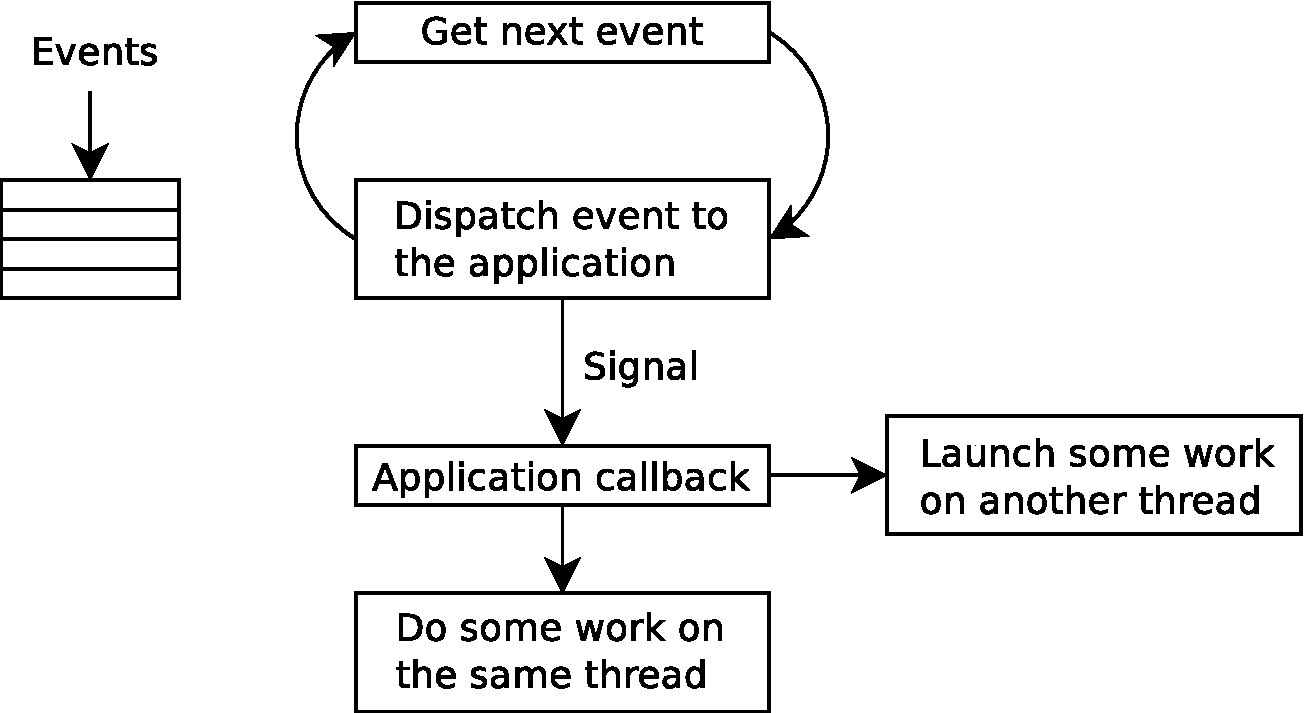
\includegraphics[width=10cm]{assets/img/event-loop.pdf}
    \caption{Estructura de una aplicación impulsada por eventos, con un bucle de eventos principal}
    \label{glib-event-loop}
  \end{center}
\end{figure}

Las aplicaciones actuales a menudo se basan en eventos. Para las aplicaciones GUI, hay muchas fuentes de eventos: una pulsación de tecla, un clic del mouse, un gesto táctil, un mensaje de otra aplicación, un cambio en el sistema de archivos, estar conectado o desconectado de la red, etc. Una aplicación necesita reaccionar a esos eventos. Por ejemplo, cuando se presiona una tecla cuando una entrada de texto tiene el foco, el carácter debe insertarse y mostrarse en la pantalla.

Pero la programación dirigida por eventos también se aplica a los daemons. La comunicación entre procesos también ocurre entre daemons y aplicaciones. Un daemon podría recibir un evento cuando llega un paquete a una interfaz de red. Un daemon de impresora podría recibir eventos cuando una impresora está conectada, desconectada, tiene poco papel, etc. Un daemon de montaje puede escuchar las memorias USB insertadas. Otro daemon puede escuchar las conexiones de monitores externos para reconfigurar las pantallas, y así sucesivamente.

Un programa impulsado por eventos no está estructurado de la misma manera que un programa por lotes. El trabajo a realizar por un programa por lotes se determina al principio. Luego analiza la entrada, realiza algunos cálculos sobre ella y genera un informe. Por ejemplo, la mayoría de los comandos y scripts de Unix son programas por lotes.

Entonces, ¿cómo estructurar una aplicación que necesita responder a varios eventos que pueden llegar en cualquier momento? Como sugiere el título de esta sección ... ¡con un \emph{bucle de evento principal} por supuesto! Esa es otra parte importante de GLib; Proporciona soporte básico de programación dirigida por eventos, con una abstracción de bucle de eventos principal, una implementación portátil de subprocesos y comunicación asincrónica entre subprocesos. Un bucle de eventos escucha algunas fuentes de eventos. Se asocia una prioridad con cada fuente de eventos. Cuando llega un evento, el bucle de eventos lo envía a la aplicación. El evento se puede tener en cuenta, ya sea en el mismo hilo o en otro hilo. La Figura~\ref{glib-event-loop} muestra una vista de alto nivel de lo que es un bucle de eventos principal.

La función \lstinline{main()} de una aplicación dirigida por eventos se ve así:

\begin{lstlisting}[style=GLib/GTK]
gint
main (gint   argc,
      gchar *argv[])
{
  /* Cree una ventana principal y adjunte devoluciones de llamada de senal. */

  /* Ejecute el bucle de eventos principal. */
  gtk_main ();

  return 0;
}
\end{lstlisting}

El bucle de eventos GTK tiene un nivel ligeramente más alto que la abstracción del bucle de eventos GLib. \lstinline{gtk_main()} ejecuta el ciclo de eventos principal hasta que se llama a \lstinline{gtk_main_quit()}. \lstinline{gtk_main_quit()} normalmente se llama en la devolución de llamada de la función cuando se hace clic en el botón de cierre o se activa la acción del menú Salir.

Una devolución de llamada es una función que se llama cuando se envía una señal. El sistema de señales está implementado por la biblioteca GObject. Escuchar una señal se logra con la función \lstinline{g_signal_connect()}:

\begin{lstlisting}[style=GLib/GTK]
static void
button_clicked_cb (GtkButton *button,
                   gpointer   user_data)
{
  MyObject *self = user_data;

  /* Hacer algo */
}

static void
create_button (MyObject *self)
{
  GtkButton *button;

  /* Crear boton */

  /* Adjuntar devolucion de llamada de senal */
  g_signal_connect (button,
                    "clicked",
                    G_CALLBACK (button_clicked_cb),
                    self);
}
\end{lstlisting}

Cuando se ejecuta una devolución de llamada, bloquea el bucle principal. Entonces, para no congelar la interfaz de usuario, existen dos soluciones:

\begin{enumerate}
    \item Las operaciones largas (especialmente las E/S) se pueden iniciar en otro hilo.
    \item Las operaciones largas se pueden dividir en fragmentos más pequeños, y cada fragmento se ejecuta en una iteración de bucle principal separada.
\end{enumerate}

Para la segunda solución, GLib proporciona las funciones \lstinline{g_idle_add()} y \lstinline{g_timeout_add()} (ver Listado~\ref{glib-idle-timeout}). Se llamará a una función inactiva cuando el bucle principal esté inactivo, es decir, cuando el bucle principal no tenga nada más que hacer. Se llama a una función de tiempo de espera a intervalos regulares. El valor de retorno booleano de una \lstinline{GSourceFunc} permite continuar o detener la función. Si continúa, el bucle principal volverá a llamar a la función en el siguiente tiempo de inactividad o tiempo de espera. Puede eliminar manualmente \lstinline{GSourceFunc} llamando a \lstinline{g_source_remove()}, que toma como parámetro el ID de origen devuelto por \lstinline{g_idle_add()} o \lstinline{g_timeout_add()}. Debe prestar atención para eliminar una \lstinline{GSourceFunc} cuando se destruye el objeto en el que realiza el cálculo. Por lo tanto, puede almacenar el ID de fuente en un atributo de objeto y llamar a \lstinline{g_source_remove()} en el destructor si el ID de fuente es diferente de \lstinline{0}. (Consulte la biblioteca de GObject para crear sus propias clases en C.)

\begin{lstlisting}[style=GLib/GTK, caption={Inactivos y tiempos de espera}, label=glib-idle-timeout]
#include <glib.h>

typedef gboolean (* GSourceFunc) (gpointer user_data);

guint g_idle_add (GSourceFunc function, gpointer data);
guint g_timeout_add (guint interval, GSourceFunc function, gpointer data);

gboolean g_source_remove (guint source_id);
\end{lstlisting}

\section{Otras características}

Simplemente no hay espacio para cubrir todas las funciones de GLib en este libro. Vale la pena mirar GLib cada vez que piense: ``Realmente \emph{debería} haber una función que ...''. Esta sección enumera otras características que proporciona GLib, pero \emph{no} es exhaustiva.

Parte del soporte de aplicaciones principales que no se ha mencionado aún:
\begin{itemize}
    \item \lstinline{GError}: un sistema de notificación de errores, similar a las excepciones en otros lenguajes.
    \item La función \lstinline{g_log()} le permite imprimir advertencias, mensajes, etc. con niveles de registro configurables y rutinas de impresión conectables.
\end{itemize}

Utilidades:
\begin{itemize}
    \item Un analizador de opciones de línea de comandos.
    \item Un marco de prueba unitaria.
    \item Una instalación de temporizador.
    \item Funciones calendáricas/aritméticas de fechas.
    \item Manipulación de nombre de archivo, como \lstinline{g_path_get_basename()} y \lstinline{g_path_is_absolute()}.
    \item Un analizador XML simple.
    \item Expresiones regulares compatibles con Perl.
\end{itemize}

Una selección de utilidades más pequeñas:
\begin{itemize}
    \item \lstinline{G_MAXFLOAT}, etc. equivalentes para muchos tipos numéricos.
    \item Conversiones por orden de bytes.
    \item \lstinline{G_DIR_SEPARATOR} maneja las diferencias de Windows/Unix.
    \item Rutinas de conveniencia/portabilidad para obtener el directorio de inicio del usuario, obtener el nombre de un directorio \path{/tmp} y tareas similares.
    \item \lstinline{G_VA_COPY} copia una \lstinline{va_list} de forma portátil.
    \item Numerosas macros para permitir el uso de extensiones del compilador (especialmente extensiones GCC) de forma portátil.
    \item Manipulación de campo de bits.
    \item Portable \lstinline {g_htonl()} y otras conversiones de host a red.
\end{itemize}

Y por último, pero no menos importante, otros tipos de datos interesantes:
\begin{itemize}
    \item Clases mejoradas de cadenas y matrices. Arreglos de punteros y bytes.
    \item \lstinline{GQuark} -- mapeo bidireccional de cadenas a identificadores enteros.
    \item \lstinline{GVariant} -- un tipo de datos genérico que almacena un valor junto con información sobre el tipo de ese valor.
\end{itemize}
\part{Programación orientada a objetos en C\label{oop}}

\chapter*{Introducción a la Parte II}
\setcounter{footnote}{0}

Ahora que está familiarizado con la biblioteca principal de GLib, ¿cuál es el siguiente paso? Como se explicó en la sección Ruta de aprendizaje (sección~\ref{intro-learning-path} p.~\pageref{intro-learning-path}), el seguimiento lógico es la programación orientada a objetos (OOP) en C y los conceptos básicos de GObject.

Cada widget GTK es una subclase de la clase base GObject. Entonces, conocer los conceptos básicos de GObject es importante para \emph{usar} un widget GTK u otra utilidad basada en GObject, pero también para \emph{crear} tus propias clases de GObject.

Es importante notar que aunque el lenguaje C no está orientado a objetos, es posible escribir código C ``semi-orientado a objetos'' fácilmente, sin GObject. Para fines de aprendizaje, con eso comienza esta parte. GObject es entonces más fácil de aprender. Lo que GObject agrega son más características como recuento de referencias, herencia, funciones virtuales, interfaces, señales y más.

Pero, ¿por qué seguir un estilo orientado a objetos en primer lugar? Un código orientado a objetos permite evitar variables globales. Y si ha leído algún tipo de guía de mejores prácticas de programación, sabe que \emph{debería}, si es posible, evitar las variables globales \footnote{Una variable global en C puede ser una variable \lstinline{static} declarada en el parte superior de un archivo *.c, al que se puede acceder desde cualquier función en ese archivo *.c. Esto a veces es útil, pero debe evitarse si es posible. Hay otro tipo de variable global en C: una variable \lstinline{extern} a la que se puede acceder desde cualquier archivo *.c. Este último es mucho peor que el primero.}. Porque el uso de datos globales hace que el código sea más difícil de administrar y comprender, especialmente cuando un programa se vuelve más grande. También hace que el código sea más difícil de reutilizar. En cambio, es mejor dividir un programa en partes más pequeñas e independientes, de modo que pueda concentrarse solo en una parte del código a la vez.

Esta parte del libro consta de dos capítulos:
\begin{itemize}
    \item Capítulo~\ref{oop-semi}, que explica cómo escribir sus propias clases semi-OOP;
    \item Capítulo~\ref{oop-gobject}, que explica los conceptos básicos de GObject.
\end{itemize}
\chapter{Programación semi-orientada a objetos en C}
\label{oop-semi}

En el capítulo anterior se explicó que la biblioteca principal de GLib utiliza un estilo de codificación semi-orientado a objetos. Esta sección explica lo que significa y cómo escribir su propio código con este estilo de codificación.

Una de las ideas principales de OOP es \emph{mantener los datos y el comportamiento relacionados en un solo lugar} \footnote{Esta es una de las pautas discutidas en \emph{Heurística de diseño orientado a objetos} \cite{oop-book}.} . En C, los datos se almacenan en una \lstinline{struct} y el comportamiento se implementa con funciones. Para mantenerlos en un solo lugar, los colocamos en el mismo archivo *.c, con las funciones públicas presentes en el archivo *.h correspondiente (el encabezado).

Otra idea importante de OOP es \emph{ocultar todos los datos dentro de su clase}. En C, significa que la declaración completa de \lstinline{struct} debe estar presente solo en el archivo *.c, mientras que el encabezado contiene solo un \lstinline{typedef}. Cómo se almacenan los datos dentro de la clase y qué estructuras de datos se utilizan debe seguir siendo un detalle de implementación. Un usuario de la clase no debe estar al tanto de los detalles de implementación, en su lugar, debe confiar solo en la interfaz externa, es decir, lo que está presente en el encabezado y la documentación pública. De esa manera, la implementación de la clase puede cambiar sin afectar a los usuarios de la clase, siempre que la API no cambie.

\section{Ejemplo de encabezado}

El Listado~\ref{oop-semi-spell-checker-h} p.~\pageref{oop-semi-spell-checker-h} muestra un ejemplo de un encabezado que proporciona un simple corrector ortográfico. Este es un código ficticio; si necesita un corrector ortográfico en su aplicación GTK, probablemente usaría hoy en día la biblioteca gspell \footnote{\url{https://wiki.gnome.org/Projects/gspell}}.

\lstinputlisting[language=C, caption={myapp-spell-checker.h}, label=oop-semi-spell-checker-h]{assets/code/myapp-spell-checker.h}

\subsection{Espacio de nombres del proyecto}
Lo primero a tener en cuenta es el uso del espacio de nombres `` Myapp ''. Cada símbolo del encabezado tiene como prefijo el espacio de nombres del proyecto.

Es una buena práctica elegir un espacio de nombres para su código, para evitar conflictos de símbolos en el momento del enlace. Es especialmente importante tener un espacio de nombres para una biblioteca, pero también es mejor tener uno para una aplicación. Por supuesto, el espacio de nombres debe ser único para cada base de código; por ejemplo, debe \emph{no} reutilizar los espacios de nombres ``G'' o ``Gtk'' para su aplicación o biblioteca.

\subsection{Espacio de nombres de clase}
Además, hay un segundo espacio de nombres con el nombre de la clase, aquí ``SpellChecker''. Si sigue esa convención de forma coherente, el nombre de un símbolo es más predecible, lo que facilita el trabajo con la API. El nombre de un símbolo siempre será ``espacio de nombres del proyecto'' + ``nombre de la clase'' + ``nombre del símbolo''.

\subsection{¿Minúsculas, Mayúsculas o CamelCase?}
Dependiendo del tipo de símbolo, su nombre está en mayúsculas, minúsculas o CamelCase. La convención en el mundo GLib es:
\begin{itemize}
    \item Letras mayúsculas para una constante, ya sea para un valor \lstinline{#define} o \lstinline{enum};
    \item CamelCase para un tipo \lstinline{struct} o \lstinline{enum};
    \item Minúsculas para funciones, variables, campos \lstinline{struct},…
\end{itemize}

\subsection{Incluir guardia}
El encabezado contiene el típico protector de inclusión:

\begin{lstlisting}[language=C]
#ifndef MYAPP_SPELL_CHECKER_H
#define MYAPP_SPELL_CHECKER_H

/* ... */

#endif /* MYAPP_SPELL_CHECKER_H */
\end{lstlisting}

Evita que el encabezado se incluya varias veces en el mismo archivo *.c.

\subsection{Soporte de C++}
El par \lstinline{G_BEGIN_DECLS}/\lstinline{G_END_DECLS} permite que el encabezado se incluya desde el código C ++. Es más importante para una biblioteca, pero también es una buena práctica agregar esas macros en el código de la aplicación, incluso si la aplicación no usa C ++. De esa manera, una clase de aplicación se podría mover a una biblioteca fácilmente (puede ser difícil notar que faltan las macros \lstinline{G_BEGIN_DECLS} y \lstinline{G_END_DECLS}). Y si surge el deseo, la aplicación podría trasladarse a C ++ de forma incremental.

\subsection{\#include}
\label{oop-semi-include-in-header}
Hay varias formas de organizar los \lstinline{#include} en una base de código C. La convención en GLib/GTK es que incluir un encabezado en un archivo *.c no debería requerir incluir otro encabezado de antemano \footnote{Esa es la regla general, pero existen excepciones: por ejemplo, incluir \lstinline{glib/gi18n-lib.h} requiere que se defina \lstinline{GETTEXT_PACKAGE}, este último suele estar presente en el encabezado \lstinline{config.h}.}.

\path{myapp-spell-checker.h} contiene el siguiente \lstinline{#include}:
\begin{lstlisting}
#include <glib.h>
\end{lstlisting}

Debido a que \path{glib.h} es necesario para las macros \lstinline{G_BEGIN_DECLS} y \lstinline{G_END_DECLS}, para las definiciones de tipos básicos de GLib (\lstinline{gchar}, \lstinline{gboolean}, etc.) y \lstinline{GSList}.

Si se elimina el \lstinline{#include} en \path{myapp-spell-checker.h}, cada archivo *.c que incluya \path{myapp-spell-checker.h} también debería incluir \path{glib.h} de antemano; de lo contrario, el compilador no podría compilar ese archivo *.c. Pero no queremos agregar tal requisito para los usuarios de la clase.

\subsection{Definición de tipo}
El tipo \lstinline{MyappSpellChecker} se define de la siguiente manera:

\begin{lstlisting}
typedef struct _MyappSpellChecker MyappSpellChecker;
\end{lstlisting}

La \lstinline{struct _MyappSpellChecker} se declarará en el archivo \path{myapp-spell-checker.c}. Cuando usa \lstinline{MyappSpellChecker} en otro archivo, no debería necesitar saber qué contiene \lstinline{struct}, debería usar las funciones públicas de la clase en su lugar. La excepción a la mejor práctica de OOP es cuando llamar a una función sería un problema de rendimiento, por ejemplo, para estructuras de datos de bajo nivel utilizadas para gráficos por computadora (coordenadas, rectángulos,…). Pero recuerde: \emph{la optimización prematura es la raíz de todos los males} (Donald~Knuth).

\subsection{Constructor de objetos}
\lstinline{myapp_spell_checker_new()} es el constructor de la clase. Toma un parámetro de código de idioma ---~por ejemplo \lstinline{"en_US"}~--- y devuelve una \emph{instancia} de la clase, también llamada \emph{objeto}. Lo que hace la función es simplemente asignar dinámicamente la \lstinline{estructura} y devolver el puntero. Ese valor de retorno se usa luego como el primer parámetro de las funciones restantes de la clase. En algunos lenguajes como Python, ese primer parámetro se llama parámetro \emph{self}, ya que hace referencia a `` sí mismo '', es decir, a su propia clase. Otros lenguajes orientados a objetos como Java y C ++ tienen la palabra clave \emph{this} para acceder a los datos del objeto.

Tenga en cuenta que \lstinline{myapp_spell_checker_new()} se puede llamar varias veces para crear diferentes objetos. Cada objeto tiene sus propios datos. Esa es la diferencia fundamental con las variables globales: si los datos se almacenan en variables globales, puede haber como máximo una instancia de ellos \footnote{A menos que la variable global almacene los ``objetos'' en una estructura de datos agregados como una matriz, un lista enlazada o una tabla hash, con un identificador como el parámetro ``\emph{self}'' (por ejemplo, un número entero o una cadena) para acceder a un elemento específico. Pero este es un código realmente desagradable, ¡por favor no lo hagas!}.

%POR HACER explicar new() (asignación en el montón) vs init() (asignación en la pila) y dar un ejemplo con init(). Pero el ejemplo también requiere el código *.c, por lo que quizás sea mejor agregar la explicación en una subsección posterior.

\subsection{Destructor de objetos}
\lstinline{myapp_spell_checker_free()} es el destructor de la clase. Destruye un objeto liberando su memoria y liberando otros recursos asignados.

\subsection{Otras funciones públicas}
Las funciones \lstinline{myapp_spell_checker_check_word()} y \lstinline{myapp_spell_checker_get_suggestions()} son las características disponibles de la clase. Comprueba si una palabra está escrita correctamente y obtiene una lista de sugerencias para corregir una palabra mal escrita.

El tipo de parámetro \lstinline{word_length} es \lstinline{gssize}, que es un tipo entero GLib que puede contener ---~por ejemplo~--- el resultado de \lstinline{strlen()}, y también puede contener un valor negativo ya que ---~contrario a \lstinline{gsize}~--- \lstinline {gssize} es un tipo entero \emph{con signo}. El parámetro \lstinline{word_length} puede ser \lstinline{-1} si la cadena está terminada en nul, es decir, si la cadena termina con el carácter especial \lstinline{'\0'}. El propósito del parámetro \lstinline{word_length} es poder pasar un puntero a una palabra que pertenece a una cadena más grande, sin la necesidad de llamar, por ejemplo, \lstinline{g_strndup()}.

\section{El archivo *.c correspondiente}

Veamos ahora el archivo \path{myapp-spell-checker.c}:

\vspace{0.7cm}
\lstinputlisting[style=GLib/GTK, caption={myapp-spell-checker.c}, label=oop-semi-spell-checker-c]{assets/code/myapp-spell-checker.c}

\subsection{Orden de \#include}
En la parte superior del archivo, se encuentra la lista habitual de \lstinline{#include}. Un detalle pequeño pero digno de mención es que el orden de inclusión no se eligió al azar. En cierto archivo *.c, es mejor incluir primero su archivo *.h correspondiente, y luego los otros encabezados \footnote{Excepto si tiene un archivo \path{config.h}, en ese caso debería \path{config.h}, \emph{luego} el *.h correspondiente, y luego los otros encabezados.}. Al incluir la primera \path{myapp-spell-checker.h}, si falta un \lstinline{#include} en \path{myapp-spell-checker.h}, el compilador informará un error. Como se explica en la sección~\ref{oop-semi-include-in-header} p.~\pageref{oop-semi-include-in-header}, un encabezado siempre debe tener el mínimo requerido \lstinline{#include}s para que ese encabezado se incluya a su vez.

Además, dado que \path{glib.h} ya está incluido en \path{myapp-spell-checker.h}, no es necesario incluirlo una segunda vez en \path{myapp-spell-checker.c}.

\subsection{Comentarios de GTK-Doc}
La API pública está documentada con comentarios GTK-Doc. Un comentario de GTK-Doc comienza con \lstinline{/**}, con el nombre del símbolo a documentar en la siguiente línea. Cuando nos referimos a un símbolo, existe una sintaxis especial a utilizar dependiendo del tipo de símbolo:
\begin{itemize}
    \item Un parámetro de función tiene el prefijo \lstinline{@}.
    \item El \emph{nombre} de una \lstinline{estructura} o \lstinline{enum} tiene el prefijo \lstinline{\#}.
    \item Una constante ---~por ejemplo, una \lstinline{enum} \emph{valor} ~---tiene el prefijo \lstinline{\%}.
    \item Una función tiene el sufijo \lstinline{()}.
\end{itemize}

GTK-Doc puede analizar esos comentarios especiales y generar páginas HTML que luego pueden ser navegadas fácilmente por un navegador API como Devhelp. Pero los comentarios especialmente formateados en el código no son lo único que necesita GTK-Doc, también necesita integración con el sistema de compilación de su proyecto (por ejemplo, Autotools), junto con algunos otros archivos para enumerar las diferentes páginas, describe el estructura general con la lista de símbolos y, opcionalmente, proporciona contenido adicional escrito en formato DocBook XML. Estos archivos suelen estar presentes en el directorio \path{docs/reference/}.

Describir en detalle cómo integrar el soporte GTK-Doc en su código está más allá del alcance de este libro. Para eso, debe consultar el manual de GTK-Doc~\cite{gtk-doc}.

Cada biblioteca basada en GLib debe tener una documentación GTK-Doc. Pero también es útil escribir una documentación GTK-Doc para el código interno de una aplicación. Como se explica en la sección~\ref{intro-backend-frontend-separation} p.~\pageref{intro-backend-frontend-separation}, es una buena práctica separar el backend de una aplicación de su(s) frontend(s), y escribir el backend como una biblioteca interna o, más tarde, una biblioteca compartida. Como tal, se recomienda documentar la API pública del backend con GTK-Doc, incluso si sigue siendo una biblioteca interna vinculada estáticamente. Porque cuando el código base se vuelve más grande, es de gran ayuda -- especialmente para los recién llegados -- tener una descripción general de las clases disponibles y saber cómo usar una clase sin la necesidad de comprender su implementación.

\subsection{Anotaciones de introspección de GObject}
El comentario de GTK-Doc para la función \lstinline{myapp_spell_checker_get_suggestions()} contiene anotaciones de GObject Introspection para el valor de retorno:

\begin{lstlisting}[language=C]
/**
 * ...
 * Returns: (transfer full) (element-type utf8): the list of suggestions.
 */
\end{lstlisting}

El tipo de retorno de la función es \lstinline{GSList *}, que no es suficiente para que los enlaces de idioma sepan qué contiene la lista, y cómo liberarla. \texttt{(transferencia completa)} significa que la persona que llama debe liberar completamente el valor de retorno: la lista misma \emph{y} sus elementos. \texttt{(tipo de elemento utf8)} significa que la lista contiene cadenas UTF-8.

Para obtener un valor de retorno, si la anotación de transferencia es \texttt{(contenedor de transferencia)}, la persona que llama necesita liberar solo la estructura de datos, no sus elementos. Y si la anotación de transferencia es \texttt{(transferir ninguna)}, la propiedad del contenido variable no se transfiere y, por lo tanto, la persona que llama no debe liberar el valor de retorno.

Hay muchas otras anotaciones de GObject Introspection (GI), por nombrar solo un par de otras:
\begin{itemize}
    \item \texttt{(nullable)}: el valor puede ser \lstinline{NULL};
    \item \texttt{(out)}: un parámetro de función ``out'', es decir, un parámetro que devuelve un valor.
\end{itemize}

Como puede ver, las anotaciones GI no solo son útiles para los enlaces de idiomas, sino que también recopilan información útil para el programador de C.

Para obtener una lista completa de anotaciones GI, consulte la wiki de GObject Introspection~\cite{gobject-introspection}.

\subsection{Funciones estáticas vs funciones no estáticas}
En el código de ejemplo, puede ver que la función \lstinline{load_dictionary()} se ha marcado como \lstinline{static}. De hecho, es una buena práctica en C marcar las funciones internas como \lstinline{static}. Una función \lstinline{static} solo se puede usar en el mismo archivo *.c. Por otro lado, una función pública debe ser no estática y tener un prototipo en un encabezado.

Existe la opción de advertencia \texttt{-Wmissing-prototypes} GCC para garantizar que un fragmento de código siga esta convención \footnote{Cuando se usan las herramientas automáticas, la macro \texttt{AX\_COMPILER\_FLAGS} Autoconf habilita, entre otras cosas, esa bandera GCC.}.

Además, contrariamente a una función pública, una función \lstinline{static} no requiere que el proyecto y los espacios de nombres de la clase tengan el prefijo (aquí, \lstinline{myapp_spell_checker}).

\subsection{Programación defensiva}
Cada función pública verifica sus precondiciones con las macros de depuración de \lstinline{g_return_if_fail()} o \lstinline{g_return_val_if_fail()}, como se describe en la sección~\ref{glib-debugging-macros} p.~\pageref{glib-debugging-macros}. El parámetro \emph{self} también se verifica, para ver si no es \lstinline{NULL}, excepto por el destructor, \lstinline{myapp_spell_checker_free()}, para que sea consistente con \lstinline{free()} y \lstinline{g_free()} que acepta un parámetro \lstinline{NULL} por conveniencia.

Tenga en cuenta que las macros \lstinline{g_return} deben usarse solo para los puntos de entrada de una clase, es decir, en sus funciones públicas. Por lo general, puede asumir que los parámetros pasados a una función \lstinline{static} son válidos, especialmente el parámetro \emph{self}. Sin embargo, a veces es útil verificar un argumento de una función \lstinline{static} con \lstinline{g_assert()}, para hacer que el código sea más robusto y auto-documentado.

\subsection{Estilo de codificación}
Finalmente, vale la pena explicar algunas cosas sobre el estilo de codificación. Se le anima a utilizar desde el principio el mismo estilo de codificación para su proyecto, ya que puede ser algo difícil de cambiar después. Si cada programa tiene diferentes convenciones de código, es una pesadilla para alguien dispuesto a contribuir.

Aquí hay un ejemplo de una definición de función:

\begin{lstlisting}[language=C]
gboolean
myapp_spell_checker_check_word (MyappSpellChecker *checker,
                                const gchar       *word,
                                gssize             word_length)
{
  /* ... */
}
\end{lstlisting}

Vea cómo se alinean los parámetros: hay un parámetro por línea, con el tipo alineado en el paréntesis de apertura y con los nombres alineados en la misma columna. Algunos editores de texto se pueden configurar para hacerlo automáticamente.

Para una función \emph{call}, si poner todos los parámetros en la misma línea da como resultado una línea demasiado larga, los parámetros también deben estar alineados entre paréntesis, para que el código sea más fácil de leer:

\begin{lstlisting}[language=C]
  function_call (one_param,
                 another_param,
                 yet_another_param);
\end{lstlisting}

A diferencia de otros proyectos como el kernel de Linux, no existe realmente un límite en la longitud de la línea. Un código basado en GObject puede tener líneas bastante largas, incluso si los parámetros de una función están alineados entre paréntesis. Por supuesto, si una línea termina en, digamos, la columna 120, podría significar que hay demasiados niveles de sangría y que debería extraer el código en funciones intermedias.

El tipo de retorno de una función \emph{definition} está en la línea anterior que el nombre de la función, por lo que el nombre de la función está al principio de la línea. Al escribir una función \emph{prototype}, el nombre de la función nunca debe estar al principio de una línea, idealmente debe estar en la misma línea que el tipo de retorno \footnote{En \path{myapp-spell-checker.h}, los nombres de las funciones están sangrados con dos espacios en lugar de estar en las mismas líneas que los tipos de retorno, porque no hay suficiente espacio horizontal en la página.}. De esa manera, puede hacer una búsqueda de expresión regular para encontrar la implementación de una función, por ejemplo, con el comando de shell \shellcmd{grep}:

\begin{lstlisting}[language=bash]
$ grep -n -E "^function_name" *.c
\end{lstlisting}

O, si el código está dentro de un repositorio de Git, es un poco más conveniente de usar \lstinline[language=bash]{git grep}:

\begin{lstlisting}[language=bash]
$ git grep -n -E "^function_name"
\end{lstlisting}

Asimismo, existe una manera fácil de encontrar la declaración de una \lstinline{struct} pública. La convención es prefijar el nombre del tipo con un guión bajo al declarar la \lstinline{struct}. Por ejemplo:

\begin{lstlisting}[language=C]
/* In the header: */
typedef struct _MyappSpellChecker MyappSpellChecker;

/* In the *.c file: */
struct _MyappSpellChecker
{
  /* ... */
};
\end{lstlisting}

Como resultado, para encontrar la declaración completa del tipo \lstinline{MyappSpellChecker}, puede buscar ``\lstinline{_MyappSpellChecker}'':

\begin{lstlisting}[language=bash]
$ git grep -n _MyappSpellChecker
\end{lstlisting}

En GLib/GTK, esta convención de prefijo de subrayado se aplica normalmente a cada \lstinline{struct} que tiene una línea \lstinline{typedef} separada. La convención no se sigue a fondo cuando se usa una \lstinline{struct} en un solo archivo *.c. Y la convención generalmente no se sigue para los tipos \lstinline{enum}. Sin embargo, para su proyecto, nada le impide aplicar consistentemente la convención de prefijo de subrayado a todos los tipos.

Tenga en cuenta que existen herramientas más sofisticadas que \shellcmd{grep} para examinar una base de código C, por ejemplo, Cscope\footnote{http://cscope.sourceforge.net/}.

Para aprender más sobre el estilo de codificación usado en GLib, GTK y GNOME, lea las Pautas de programación de GNOME~\cite{gnome-programming-guidelines}.
\chapter{Una suave introducción a GObject}
\label{oop-gobject}

En el capítulo anterior hemos aprendido a escribir código semi-orientado a objetos en C. Así es como se escriben las clases en GLib core. GObject avanza varios pasos en la programación orientada a objetos, con herencia, interfaces, funciones virtuales, etc. GObject también simplifica el paradigma de programación dirigida por eventos, con señales y propiedades.

Se recomienda crear sus propias clases de GObject para escribir una aplicación GLib/GTK. Desafortunadamente, el código es un poco detallado, porque el lenguaje C no está orientado a objetos. El código repetitivo es necesario para algunas funciones, pero no tenga miedo, existen herramientas y scripts para generar el modelo repetitivo.

Sin embargo, este capítulo da un paso atrás del capítulo anterior, es solo una pequeña introducción a GObject; explicará las cosas esenciales para saber cómo \emph{usar} una clase GObject existente (como todos los widgets y clases GTK en GIO). No explicará cómo \emph{crear} sus propias clases de GObject, porque ya está bien cubierto en el manual de referencia de GObject, y el objetivo de este libro no es duplicar todo el contenido de los manuales de referencia, el objetivo es más para que sirva de guía de introducción.

Entonces, para obtener información más detallada sobre GObject y saber cómo crear subclases, la documentación de referencia de GObject contiene capítulos introductorios: ``\emph{Conceptos}'' y ``\emph{Tutorial}'', disponibles en:

\url{https://docs.gtk.org/gobject/}

Para explicar ciertos conceptos, se toman algunos ejemplos de GTK o GIO. Al leer este capítulo, se le anima a abrir Devhelp en paralelo, para mirar la referencia de API y ver por sí mismo cómo se documenta una biblioteca basada en GObject. El objetivo es que seas autónomo y puedas aprender cualquier clase nueva de GObject, ya sea en GIO, GTK o cualquier otra biblioteca.

\section{Herencia}
\label{oop-gobject-inheritance}

Un concepto importante de OOP es la herencia. Una clase puede ser una subclase de una clase principal. La subclase hereda las características de la clase padre, extendiendo o anulando su comportamiento.

La biblioteca GObject proporciona la clase base \lstinline{GObject}. Cada clase en GIO y GTK hereda, directa o indirectamente, de la clase base \lstinline{GObject}. Al mirar una clase basada en GObject, la documentación (si está escrita con GTK-Doc) siempre contiene una \emph{Jerarquía de objetos}. Por ejemplo, \lstinline{GtkApplication} tiene la siguiente jerarquía de objetos:

\begin{verbatim}
GObject
└── GApplication
    └── GtkApplication
\end{verbatim}

Significa que cuando crea un objeto \lstinline{GtkApplication}, también tiene acceso a las funciones, señales y propiedades de \lstinline{GApplication} (implementado en GIO) y \lstinline{GObject}. Por supuesto, las funciones \lstinline{g_application_*} toman como primer argumento una variable de tipo ``\lstinline{GApplication *}'', no ``\lstinline{GtkApplication *}''. Para convertir la variable en el tipo correcto, la forma recomendada es usar la macro \lstinline{G_APPLICATION()}. Por ejemplo:

\begin{lstlisting}[style=GLib/GTK]
GtkApplication *app;

g_application_mark_busy (G_APPLICATION (app));
\end{lstlisting}

\section{Macros de GObject}

Cada clase de GObject proporciona un conjunto de macros estándar. La macro \lstinline{G_APPLICATION()} como se demostró en la sección anterior es una de las macros estándar proporcionadas por la clase \lstinline{GApplication}.

No todas las macros estándar de GObject se explicarán aquí, solo las macros útiles para \emph{usar} un GObject de una manera básica. Las otras macros son más avanzadas y generalmente son útiles solo cuando se subclasifica una clase GObject, cuando se crea una propiedad o una señal, o cuando se reemplaza una función virtual.

Cada clase GObject define una macro de la forma \lstinline{NAMESPACE_CLASSNAME(object)}, que convierte la variable al tipo ``\lstinline{NamespaceClassname *}'' y comprueba en tiempo de ejecución si la variable contiene correctamente un \lstinline{NamespaceClassname} objeto o una subclase del mismo. Si la variable es \lstinline{NULL} o contiene un objeto incompatible, la macro imprime un mensaje de advertencia crítico en la consola y devuelve NULL.

Un elenco estándar también funciona, pero la mayoría de las veces no se recomienda porque no hay comprobaciones de tiempo de ejecución:

\begin{lstlisting}[style=GLib/GTK]
GtkApplication *app;

/* No recomendado */
g_application_mark_busy ((GApplication *) app);
\end{lstlisting}

Otra macro útil cuando se usa un GObject es \lstinline{NAMESPACE_IS_CLASSNAME(object)}, que devuelve \lstinline{TRUE} si la variable es un objeto \lstinline{NamespaceClassname} o una subclase del mismo.

% POR HACER mostrar un ejemplo de una función que verifica sus argumentos con g_return?

\section{Interfaces}

Con GObject es posible crear interfaces. Una interfaz es solo una API, no contiene la implementación. Una clase GObject puede implementar una o varias interfaces. Si una clase GObject está documentada con GTK-Doc, la documentación contendrá una sección \emph{Interfaces implementadas}.

Por ejemplo, GTK contiene la interfaz \lstinline{GtkOrientable} que es implementada por muchos widgets y permite establecer la orientación: horizontal o vertical.

Las dos macros explicadas en la sección anterior también funcionan para interfaces. Un ejemplo con \lstinline{GtkGrid}:

\begin{lstlisting}[style=GLib/GTK]
GtkWidget *vgrid;

vgrid = gtk_grid_new ();
gtk_orientable_set_orientation (GTK_ORIENTABLE (vgrid),
                                GTK_ORIENTATION_VERTICAL);
\end{lstlisting}

Entonces, cuando busca una determinada característica en la API para una cierta clase de GObject, la característica se puede ubicar en tres lugares diferentes:
\begin{itemize}
    \item En la propia clase GObject;
    \item En una de las clases padre en \emph{Jerarquía de objetos};
    \item O en una de las \emph{Interfaces implementadas}.
\end{itemize}

\section{Recuento de referencias}

La gestión de la memoria de las clases de GObject se basa en \emph{recuento de referencias}. Una clase GObject tiene un contador:
\begin{itemize}
    \item Cuando se crea el objeto, el contador es igual a uno;
    \item \lstinline{g_object_ref()} incrementa el contador;
    \item \lstinline{g_object_unref()} disminuye el contador;
    \item Si el contador llega a cero, el objeto se libera.
\end{itemize}

Permite almacenar el GObject en varios lugares sin necesidad de coordinar cuándo liberar el objeto.

\subsection{Evitar ciclos de referencia con referencias débiles}

Si el objeto A hace referencia al objeto B y el objeto B hace referencia al objeto A, hay un ciclo de referencia y los dos objetos nunca se liberarán. Para evitar ese problema, existe el concepto de referencias ``débiles''. Al llamar a \lstinline{g_object_ref()}, es una referencia ``sólida''. Entonces, en una dirección hay una referencia fuerte, y en la otra dirección debe haber una referencia débil (o ninguna referencia).

\begin{figure}[H]
  \begin{center}
    
\includegraphics[scale=0.75]{assets/img/weak-ref.pdf}
    \caption{Usar una referencia débil para romper el ciclo de referencia entre A y B.}
    \label{oop-gobject-weak-ref-schema}
  \end{center}
\end{figure}

En la Figura~\ref{oop-gobject-weak-ref-schema} podemos ver que el objeto A tiene una fuerte referencia al objeto B, y el objeto B tiene una débil referencia al objeto A.

Se puede crear una referencia débil con \lstinline{g_object_add_weak_pointer()} o \lstinline{g_object_weak_ref()}. Al igual que con las referencias fuertes, es importante liberar la referencia cuando ya no se necesite, generalmente en el destructor de clases. Una referencia débil debe eliminarse con \lstinline{g_object_remove_weak_pointer()} o \lstinline{g_object_weak_unref()}. Entonces, en la Figura~\ref{oop-gobject-weak-ref-schema}, el destructor de la clase B debe eliminar la referencia débil si aún no lo ha hecho.

\subsection{Referencias flotantes}

Cuando una clase GObject hereda de \lstinline{GInitiallyUnowned} (que es el caso de \lstinline{GtkWidget}), el objeto inicialmente tiene una referencia \emph{floating}. Se debe llamar a \lstinline{g_object_ref_sink()} para convertir esa referencia flotante en una referencia normal y fuerte.

Cuando un GObject hereda de \lstinline{GInitiallyUnowned}, significa que GObject debe incluirse en algún tipo de contenedor. El contenedor luego asume la propiedad de la referencia flotante, llamando a \lstinline{g_object_ref_sink()}. Permite simplificar el código, para eliminar la necesidad de llamar a \lstinline{g_object_unref()} después de incluir el objeto en el contenedor.

El Listado~\ref{oop-gobject-mem-management-normal} p.~\pageref{oop-gobject-mem-management-normal} muestra cómo se maneja la administración de memoria con un GObject normal. Compare esto con el Listado~\ref{oop-gobject-mem-management-floating}, que muestra cómo se maneja la administración de memoria con un GObject derivado de \lstinline{GInitiallyUnowned}. La diferencia es que \lstinline{g_object_unref()} no se llama en el último Listado, por lo que acorta el código.

\begin{lstlisting}[style=GLib/GTK, caption={Gestión de la memoria de GObjects normales.}, label=oop-gobject-mem-management-normal]
/* GObject normal */

a_normal_gobject = normal_gobject_new ();
/* a_normal_gobject tiene ahora un recuento de referencia de 1. */

container_add (container, a_normal_gobject);
/* a_normal_gobject tiene ahora un recuento de referencia de 2. */

/* Ya no necesitamos un a_normal_gobject, por lo que lo anulamos. */
g_object_unref (a_normal_gobject);
/* a_normal_gobject tiene ahora un recuento de referencia de 1. */
\end{lstlisting}

\begin{lstlisting}[style=GLib/GTK, caption={Gestión de memoria de GObjects derivados de \lstinline{GInitiallyUnowned}.}, label=oop-gobject-mem-management-floating]
/* Objeto GInitiallyUnowned, p. Ej. un GtkWidget */

widget = gtk_entry_new ();
/* widget tiene ahora solo una referencia flotante. */

gtk_container_add (container, widget);
/* El contenedor ha llamado a g_object_ref_sink(), tomando
 * posesion de la referencia flotante. El codigo esta
 * simplificado porque no debemos llamar a g_object_unref().
 */
\end{lstlisting}

Entonces, es importante saber si un GObject hereda de \lstinline{GInitiallyUnowned} o no. Para eso, debe mirar la \emph{Object Hierarchy}, por ejemplo, \lstinline{GtkEntry} tiene la siguiente jerarquía:

\begin{verbatim}
GObject
└── GInitiallyUnowned
    └── GtkWidget
        └── GtkEntry
\end{verbatim}

\section{Señales y propiedades}
\label{oop-gobject-signals-and-properties}

Una clase GObject puede emitir señales. Con el bucle de eventos principal GLib (explicado anteriormente en la sección~\ref{glib-main-event-loop} p.~\pageref{glib-main-event-loop}), esta es la base para la programación dirigida por eventos. Un ejemplo de señal es cuando el usuario hace clic en un botón. La aplicación conecta una función de devolución de llamada a la señal para realizar la acción deseada cuando ocurre el evento.

Otro concepto de GObject son las \emph{propiedades}, que está relacionado con las señales. Una propiedad es básicamente una variable de instancia coronada con una señal de \lstinline{"notify"} que se emite cuando cambia su valor. Un buen ejemplo de una propiedad es el estado de un botón de verificación, es decir, un valor booleano que describe si el botón está actualmente marcado o no. Cuando el estado cambia, se envía la señal \lstinline{"notify"}.

Para crear sus propias señales o propiedades, se debe crear una subclase GObject. Como se explicó en la introducción de este capítulo, esto está más allá del alcance de este libro, pero debe tener en cuenta que, por supuesto, es posible y recomendable crear sus propias señales o propiedades. De hecho, crear una señal o propiedad de GObject es una buena manera de implementar el patrón de diseño Observer \cite{design-patterns-book}; es decir, uno o varios objetos \emph{observando} cambios de estado de otro objeto, conectando devoluciones de llamada de función. El objeto que \emph{emite} la señal no sabe qué objetos \emph{reciben} la señal. GObject solo realiza un seguimiento de la lista de devoluciones de llamada para llamar. Entonces, agregar una señal permite desacoplar clases.

\subsection{Conexión de una función de devolución de llamada a una señal}

Para hacer las cosas más concretas, si observa la documentación de \lstinline{GtkButton}, verá que proporciona la señal \lstinline{"clicked"}. Para realizar la acción deseada cuando se emite la señal, una o más funciones de devolución de llamada deben estar conectadas de antemano.

Para conectar una devolución de llamada a una señal, se puede usar la función \lstinline{g_signal_connect()}, o una de las otras funciones \lstinline{g_signal_connect_*()}:
\begin{itemize}
  \item \lstinline{g_signal_connect()}
  \item \lstinline{g_signal_connect_after()}
  \item \lstinline{g_signal_connect_swapped()}
  \item \lstinline{g_signal_connect_data()}
  \item \lstinline{g_signal_connect_object()}
  \item Y algunas más avanzadas.
\end{itemize}

El Listado~\ref{oop-gobject-gtkbutton-clicked} p.~\pageref{oop-gobject-gtkbutton-clicked} muestra el prototipo de la señal \lstinline{GtkButton::clicked} \footnote{La convención cuando se hace referencia a una señal de GObject es ``\lstinline{ClassName::signal-name}''. Así es como se documenta con los comentarios de GTK-Doc.}.

\begin{lstlisting}[style=GLib/GTK, caption={El prototipo de la señal \lstinline{GtkButton::clicked}.}, label=oop-gobject-gtkbutton-clicked]
void
user_function (GtkButton *button,
               gpointer   user_data);
\end{lstlisting}

Cuando se usa \lstinline{g_signal_connect()}, la función de devolución de llamada debe tener el mismo prototipo que el prototipo de señal. Muchas señales tienen más argumentos y algunas señales devuelven un valor. Si la devolución de llamada tiene un prototipo incompatible, sucederán cosas malas, habrá errores o bloqueos aleatorios.

El Listado~\ref{oop-gobject-connect-to-signal} p.~\pageref{oop-gobject-connect-to-signal} muestra un ejemplo de cómo usar \lstinline{g_signal_connect()}.

\begin{lstlisting}[style=GLib/GTK, caption={Cómo conectarse a una señal}, label=oop-gobject-connect-to-signal]
static void
button_clicked_cb (GtkButton *button,
                   gpointer   user_data)
{
  MyClass *my_class = MY_CLASS (user_data);

  g_message ("Boton pulsado!");
}

static void
create_button (MyClass *my_class)
{
  GtkButton *button;

  /* Crea el boton */
  /* ... */

  /* Conectar la funcion de devolucion de llamada */
  g_signal_connect (button,
                    "clicked",
                    G_CALLBACK (button_clicked_cb),
                    my_class);
}
\end{lstlisting}

La macro \lstinline{G_CALLBACK()} es necesaria porque \lstinline{g_signal_connect()} es genérica: se puede usar para conectarse a cualquier señal de cualquier clase de GObject, por lo que el puntero de función debe ser convertido.

Hay dos convenciones principales para nombrar funciones de devolución de llamada:
\begin{itemize}
  \item Termine el nombre de la función con ``\lstinline{cb}'', atajo de ``callback''. Por ejemplo: \lstinline{button_clicked_cb()} como en el ejemplo de código anterior.
  \item Inicie el nombre de la función con ``\lstinline{on}''. Por ejemplo: \lstinline{on_button_clicked()}.
\end{itemize}

Con una de esas convenciones de nomenclatura --- y con el parámetro \lstinline{gpointer user_data}, que siempre es el último parámetro --- es fácil reconocer que una función es una devolución de llamada.

El lenguaje C permite escribir una firma de función de devolución de llamada diferente --- pero compatible ---, aunque no se considera universalmente como algo bueno:
\begin{itemize}
  \item Uno o más de los \emph{últimos} argumentos de la función se pueden omitir si no se utilizan. Pero como se explicó anteriormente, el argumento \lstinline{gpointer user_data} permite reconocer fácilmente que la función es efectivamente una devolución de llamada \footnote{Al igual que con los lenguajes naturales, la redundancia permite comprender mejor y más rápidamente lo que leemos o escuchamos.}.
  \item Los tipos de argumentos se pueden modificar a un tipo compatible: p. Ej. otra clase en la jerarquía de herencia, o en el ejemplo anterior, reemplazando ``\lstinline{gpointer}'' por ``\lstinline{MyClass *}'' (pero hacer eso hace que el código sea un poco menos robusto porque no se llama a la macro \lstinline{MY_CLASS()}).
\end{itemize}

\subsection{Desconexión de controladores de señales}

En el Listado~\ref{oop-gobject-connect-to-signal}, se llama a \lstinline{button_clicked_cb()} cada vez que el objeto \lstinline{button} emite la señal \lstinline{"clicked"}. Si el objeto \lstinline{button} todavía está vivo después de que \lstinline{my_class} se haya liberado, cuando la señal se emita nuevamente habrá un pequeño problema ... Entonces, en el destructor de \lstinline{MyClass}, el manejador de señales (es decir, la devolución de llamada) debe desconectarse. ¿Como hacer eso?

Las funciones \lstinline{g_signal_connect*()} en realidad devuelven un ID del manejador de señales, como un entero \lstinline{gulong} siempre mayor que 0 (para conexiones exitosas). Al almacenar ese ID, es posible desconectar ese manejador de señal específico con la función \lstinline{g_signal_handler_disconnect()}.

A veces también queremos desconectar el controlador de señales simplemente porque ya no estamos interesados en el evento.

El Listado~\ref{oop-gobject-disconnect-signal} muestra un ejemplo completo de cómo desconectar un manejador de señales cuando se libera su argumento \lstinline{user_data}. Volvemos a un ejemplo con un corrector ortográfico, porque el ejemplo con el botón GTK no se ajusta bien a la situación \footnote{La mayoría de las veces, un widget GTK no vive más tiempo que el contenedor al que se agrega, y el El objeto que escucha la señal del widget suele ser el propio contenedor. Entonces, si el widget muere al mismo tiempo que el contenedor, no es posible que el widget envíe una señal mientras su contenedor ya ha sido destruido. En ese caso, no tiene sentido desconectar la señal en el destructor del contenedor, ya que en ese punto el widget ya está liberado; y es más difícil para un objeto muerto enviar una señal \footnotemark.}.
% GObject es aburrido, por lo que un poco de humor no duele, una nota al pie dentro de una nota al pie, recepción al pie :-)
\footnotetext{Cuando digo que es más difícil, en realidad es imposible, por supuesto.}

El argumento de devolución de llamada \lstinline{user_data} es una instancia de \lstinline{MyTextView}, con \lstinline{MyTextView} implementado con un estilo semi-OOP. Dado que el objeto del corrector ortográfico puede vivir más tiempo que la instancia de \lstinline{MyTextView}, la señal debe desconectarse en el destructor \lstinline{MyTextView}.

\vspace{0.7cm}
\lstinputlisting[style=GLib/GTK, caption={Desconectar un manejador de señales cuando se libera su argumento \lstinline{user_data}.}, label=oop-gobject-disconnect-signal]{assets/code/disconnect-signal.c}

En realidad, hay otras funciones de \lstinline{g_signal_handler*()} que permiten desconectar los manejadores de señales:
\begin{itemize}
  \item \lstinline{g_signal_handlers_disconnect_by_data()}
  \item \lstinline{g_signal_handlers_disconnect_by_func()}
  \item \lstinline{g_signal_handlers_disconnect_matched()}
\end{itemize}

Habría sido posible utilizar una de las funciones anteriores en el Listado~\ref{oop-gobject-disconnect-signal}, y habría evitado la necesidad de almacenar \lstinline{word_added_to_personal_handler_id}. La función básica \lstinline{g_signal_handler_disconnect()} se ha utilizado con fines de aprendizaje.

Tenga en cuenta también que si \lstinline{MyTextView} fuera una clase GObject, habría sido posible conectarse a la señal del corrector ortográfico con \lstinline{g_signal_connect_object()}, y habría eliminado por completo la necesidad de desconectar manualmente el controlador de señal en el destructor \lstinline{MyTextView}. Una (pequeña) razón más para aprender a crear subclases de GObject.

\subsection{Propiedades}

Si ha mirado la referencia de la API GTK o GIO, debe haber notado que algunas clases de GObject tienen una o más \emph{propiedades}. Una propiedad es como una variable de instancia, también llamada ``attribute'', pero es diferente en el contexto de GObject porque tiene propiedades interesantes adicionales \footnote{Pun intencionado.}.

Como se dijo anteriormente al comienzo de la sección~\ref{oop-gobject-signals-and-properties} p.~\pageref{oop-gobject-signals-and-properties}, un buen ejemplo de una propiedad es el estado de un botón de verificación, es decir, un valor booleano que describe si el botón está actualmente marcado o no. Si ya conoce un poco de GTK, es posible que haya descubierto que hay un botón de verificación disponible con el widget \lstinline{GtkCheckButton}. Pero había una pequeña trampa si quería encontrar la propiedad de la que estaba hablando, porque la propiedad está implementada en la clase padre \lstinline{GtkToggleButton}: la propiedad \lstinline{GtkToggleButton:active} \footnote{De la misma manera como las señales se documentan con GTK-Doc como ``\lstinline{ClassName::signal-name}'', las propiedades se documentan como ``\lstinline{ClassName:property-name}''.}.

\subsubsection{La señal \lstinline{notify} }

El atributo principal \footnote{Pun también intencionado.} De una propiedad ---~además de representar un valor~--- es que la clase GObject emite la señal \lstinline{GObject::notify} cuando cambia el valor de una propiedad.

Hay un concepto de señales GObject que aún no se ha explicado y se usa con la señal \lstinline{GObject::notify}: cuando se emite una señal, se puede proporcionar un \emph{detail}. En el caso de la señal de notificación, el detalle es el nombre de la propiedad cuyo valor ha cambiado. Dado que solo hay una señal para todas las propiedades, gracias al \emph{detail} es posible conectar una devolución de llamada para recibir una notificación solo cuando una determinada propiedad haya cambiado. Si el \emph{detail} no se proporciona al conectar la devolución de llamada, la devolución de llamada se llamará cuando \emph{cualquiera} de las propiedades del objeto cambie, lo que generalmente no es lo que se desea.

Será más claro con un ejemplo. El Listado~\ref{oop-gobject-connect-to-notify} p.~\pageref{oop-gobject-connect-to-notify} muestra cómo conectarse a la señal de notificación. Tenga en cuenta que en lugar de conectarse a la señal detallada \lstinline{"notify::active"}, en realidad es más conveniente utilizar la señal \lstinline{GtkToggleButton::toggled}. Hay mejores casos de uso en el mundo real en los que es necesario conectarse a la señal de notificación, pero al menos el Listado~\ref{oop-gobject-connect-to-notify} es, con suerte, comprensible con solo un conocimiento limitado de GTK (y si mira la documentación en Devhelp en paralelo).

\begin{lstlisting}[style=GLib/GTK, caption={Conexión a la señal de notificación para escuchar cambios en la propiedad.}, label=oop-gobject-connect-to-notify]
/* If you look at the notify signal documentation, the first parameter
 * has the type GObject, not GtkCheckButton. Since GtkCheckButton is a
 * sub-class of GObject, the C language allows to write GtkCheckButton
 * directly.
 */
static void
check_button_notify_cb (GtkCheckButton *check_button,
                        GParamSpec     *pspec,
                        gpointer        user_data)
{
  /* Called each time that any property of check_button changes. */
}

static void
check_button_notify_active_cb (GtkCheckButton *check_button,
                               GParamSpec     *pspec,
                               gpointer        user_data)
{
  MyWindow *window = MY_WINDOW (user_data);
  gboolean active;

  active = gtk_toggle_button_get_active (GTK_TOGGLE_BUTTON (check_button));
  gtk_widget_set_visible (window->side_panel, active);
}

static GtkWidget *
create_check_button (MyWindow *window)
{
  GtkWidget *check_button;

  check_button = gtk_check_button_new_with_label ("Show side panel");

  /* Connect without the detail. */
  g_signal_connect (check_button,
                    "notify",
                    G_CALLBACK (check_button_notify_cb),
                    NULL);

  /* Connect with the detail, to be notified only when
   * the GtkToggleButton:active property changes.
   */
  g_signal_connect (check_button,
                    "notify::active",
                    G_CALLBACK (check_button_notify_active_cb),
                    window);

  return check_button;
}
\end{lstlisting}

\subsubsection{Vinculaciones de propiedad}

Otro aspecto útil de las propiedades es que dos propiedades se pueden vincular fácilmente: cuando una propiedad cambia, la otra se actualiza para tener el mismo valor. Lo mismo se puede lograr con la señal \lstinline{"notify"}, pero existen funciones de nivel superior.

Se pueden vincular dos propiedades de varias formas con una de las funciones \lstinline{g_object_bind_property*()}. El Listado~\ref{oop-gobject-binding-properties} muestra una implementación más simple del Listado~\ref{oop-gobject-connect-to-notify}; el código es equivalente, pero usa la función \lstinline{g_object_bind_property()}.

\vspace{0.7cm}
\begin{lstlisting}[style=GLib/GTK, caption={Vinculando dos propiedades.}, label=oop-gobject-binding-properties]
static GtkWidget *
create_check_button (MyWindow *window)
{
  GtkWidget *check_button;

  check_button = gtk_check_button_new_with_label ("Show side panel");

  /* When the GtkToggleButton:active property of check_button changes,
   * the GtkWidget:visible property of window->side_panel is updated to
   * have the same boolean value.
   *
   * It would be useful to add G_BINDING_SYNC_CREATE to the flags, but
   * in that case the code would not be equivalent to the previous
   * code Listing.
   */
  g_object_bind_property (check_button, "active",
                          window->side_panel, "visible",
                          G_BINDING_DEFAULT);

  return check_button;
}
\end{lstlisting}
\part{GTK}
\chapter{Ejemplo de una arquitectura de código de aplicación GTK}
\label{gtk-app-arch}

\emph{Este capítulo no está completamente terminado, puede ser difícil de entender sin ningún conocimiento sobre GTK u otro conjunto de herramientas de widgets. Y el capítulo no está bien integrado con los otros capítulos, la introducción y los capítulos de lectura adicional no se han adaptado, por ejemplo. Este capítulo se distribuye con la esperanza de que sea útil, pero SIN NINGUNA GARANTÍA; incluso sin la garantía implícita de COMERCIABILIDAD o APTITUD PARA UN PROPÓSITO EN PARTICULAR.}

%FIXME: vuelve a explicar qué es un "widget" y un "contenedor". Y agregue un glosario al final.

Para cualquier proyecto de programación, es importante diseñar correctamente la arquitectura de código general. Con Programación Orientada a Objetos, significa definir las clases principales. Este capítulo explica un buen ejemplo de una arquitectura de código para una aplicación GTK, observando una vista simplificada del editor de texto gedit \footnote{\url{https://wiki.gnome.org/Apps/Gedit}}.

gedit tiene una interfaz de documento con pestañas: se pueden abrir varios archivos en la misma ventana de gedit, en diferentes pestañas. Como veremos, esto se refleja en la arquitectura del código.

La Figura~\ref{fig:gedit-architecture} p.~\pageref{fig:gedit-architecture} muestra el esquema de la clase. Cada clase gedit en el esquema es una subclase de una clase GTK o GtkSourceView. (GtkSourceView \footnote{\url{https://wiki.gnome.org/Projects/GtkSourceView}} es una biblioteca que extiende el widget \lstinline{GtkTextView}; \lstinline{GtkTextView} es parte de GTK).

Repasaremos el esquema de la clase, explicando las clases paso a paso, comenzando por la parte superior. Esto permitirá presentar algunas de las clases GTK más importantes, no describiéndolas en detalle con muchos ejemplos de código, sino dando una descripción general de alto nivel.

\begin{figure}
  \begin{center}
    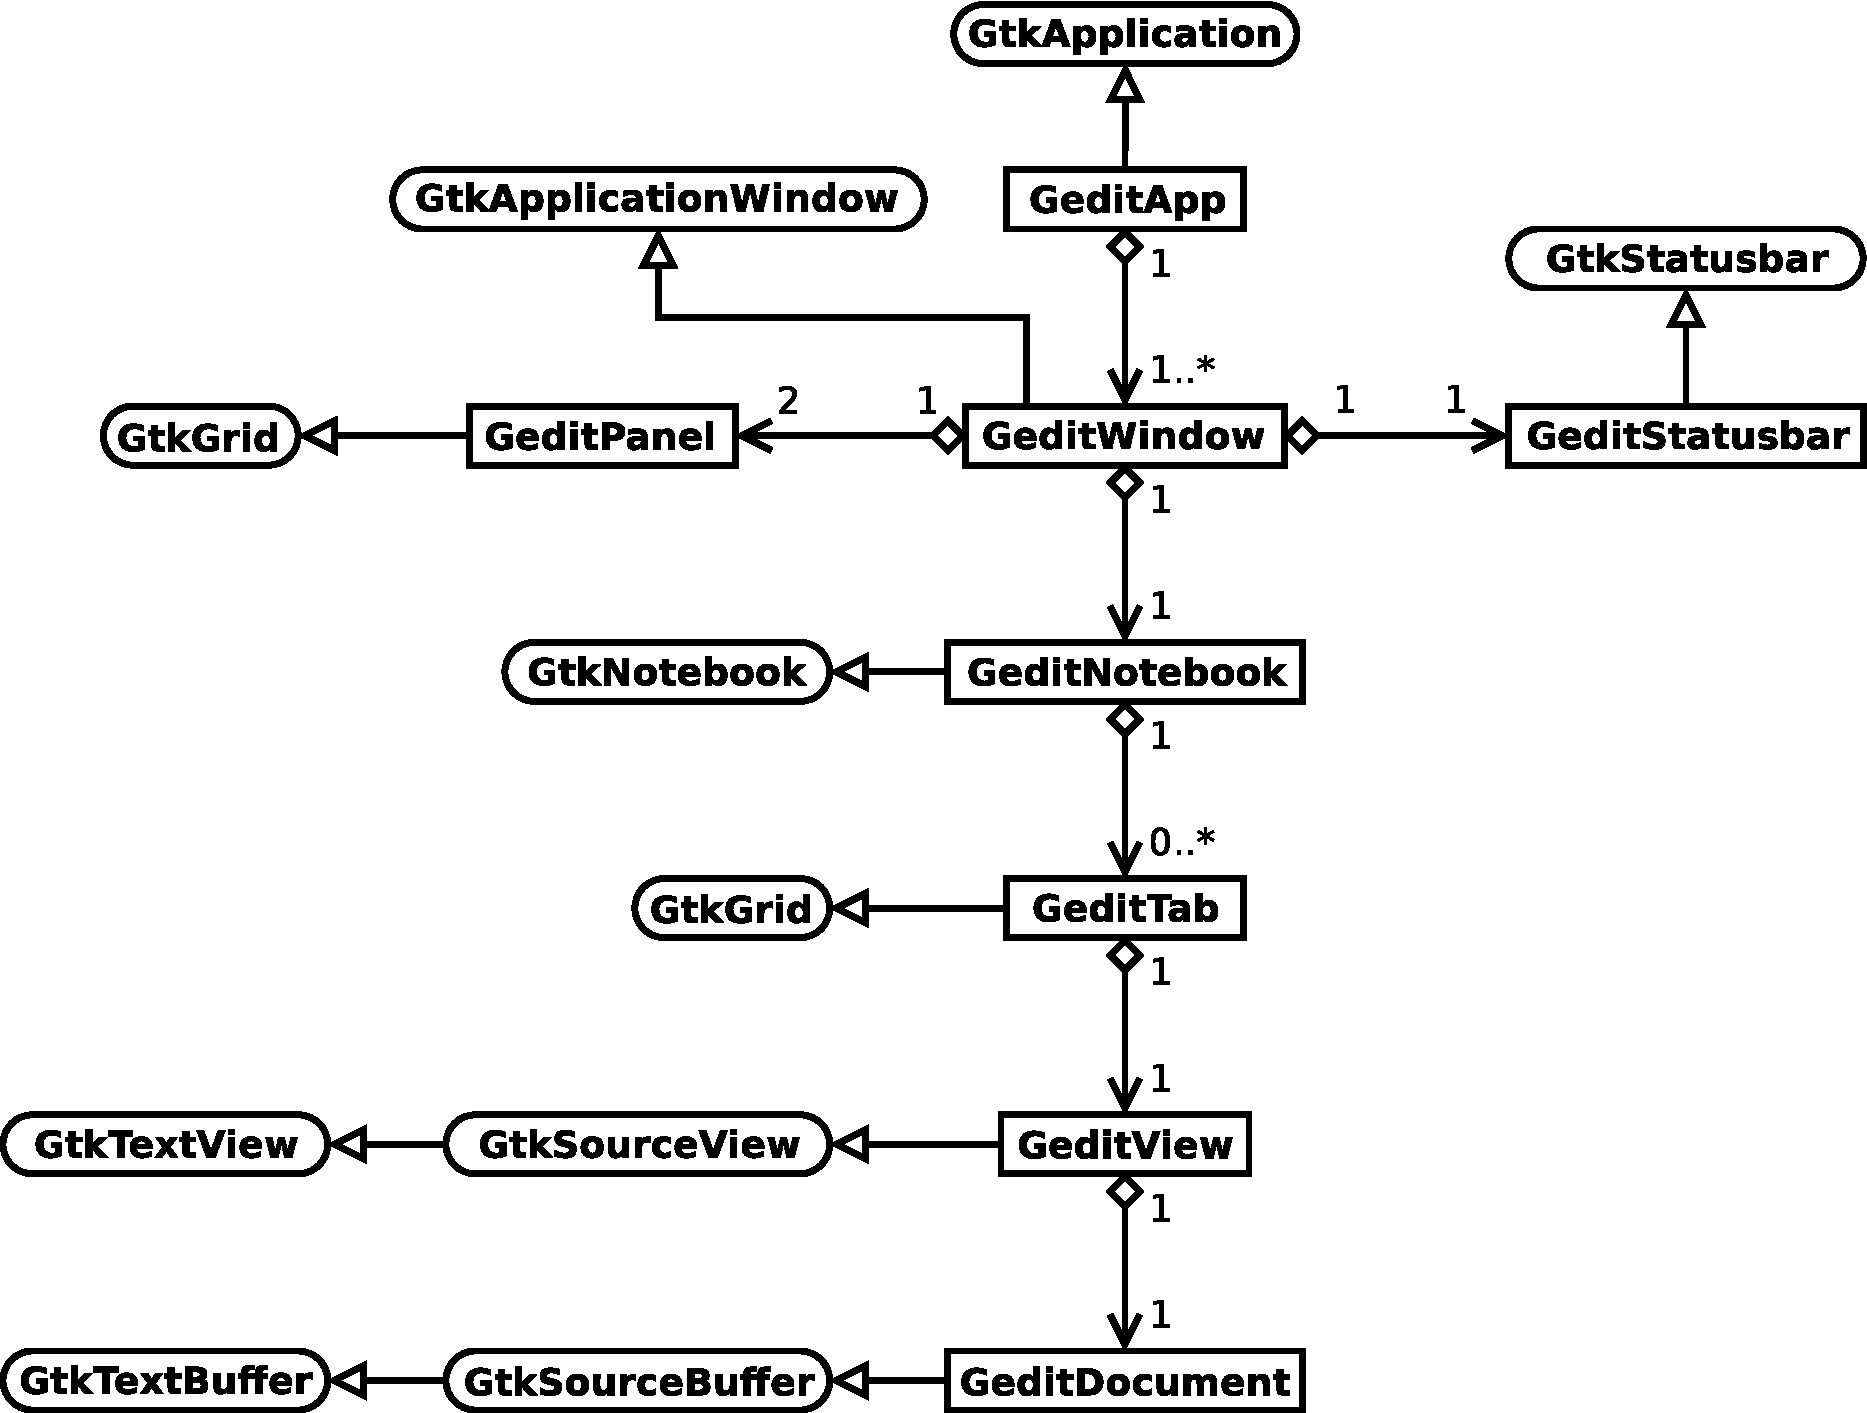
\includegraphics[width=\textwidth]{assets/img/gedit-architecture.pdf}
    \caption{Arquitectura de código simplificada del editor de texto gedit}
    \label{fig:gedit-architecture}
  \end{center}
\end{figure}

\section{La función main() y GeditApp}

Aunque no está representado en el esquema, el punto de entrada de una aplicación GTK --~como para todos los programas en C~-- es la función \lstinline{main()}. Para crear una aplicación GTK, lo principal que se debe hacer en \lstinline{main()} es crear una instancia de \lstinline{GtkApplication}, o una subclase de la misma. En el esquema vemos que \lstinline{GeditApp} es una subclase de \lstinline{GtkApplication}, por lo que la función \lstinline{main()} de gedit crea un objeto \lstinline{GeditApp}.

\lstinline{GtkApplication} es la clase que contiene y representa la aplicación completa. Por lo general, solo hay una instancia de \lstinline{GtkApplication} por proceso, por lo que puede considerarse una clase singleton. Lo que contiene \lstinline{GtkApplication} son \emph{windows}, por ejemplo, \lstinline{GeditWindow} en el caso de gedit, además de otros tipos de ventanas como ventanas de diálogo.

Ya vimos la jerarquía de clases \lstinline{GtkApplication} en la sección~\ref{oop-gobject-inheritance} p.~\pageref{oop-gobject-inheritance} al explicar la herencia POO con GObject:

\begin{verbatim}
GObject
└── GApplication
    └── GtkApplication
\end{verbatim}

\lstinline{GApplication} es parte de la biblioteca GIO e implementa las funciones que no están relacionadas con la interfaz gráfica de usuario (GUI). Entonces, para un programa que se ejecuta en la terminal, es posible usar solo \lstinline{GApplication}.

Una característica importante que proporciona \lstinline{GApplication} es la unicidad del proceso (pero puede desactivarse si no se desea). Lo que hace la unicidad del proceso es tener solo un proceso por aplicación por sesión de usuario. Para que esa característica funcione, se debe proporcionar un ID de aplicación al crear el objeto \lstinline{GApplication}. Con ese ID, \lstinline{GApplication} busca si otro proceso ya ejecuta la misma aplicación en la misma sesión de usuario; si es el caso, comunica a la instancia primaria las acciones que deben realizarse (por ejemplo, abrir una nueva ventana, o abrir un nuevo archivo en una ventana existente, etc.). Cuando las acciones se realizan en la instancia principal, el segundo proceso finaliza inmediatamente. En Linux, \lstinline{GApplication} utiliza el sistema de comunicación entre procesos (IPC) D-Bus para comunicarse entre los dos procesos.

La singularidad del proceso tiene varias ventajas, por dar algunos ejemplos concretos:
\begin{itemize}
  \item Para una aplicación con una interfaz de documento con pestañas, al hacer clic en un archivo en un administrador de archivos como Nautilus, el archivo se puede abrir en una nueva pestaña en lugar de crear cada vez una nueva ventana. Para que esto funcione, la comunicación entre procesos es necesaria de una forma u otra;
  \item Una aplicación no necesita sincronizar explícitamente su estado y datos entre diferentes procesos. En aras del argumento, digamos que en gedit el usuario puede crear `` herramientas de compilación '' personalizadas para compilar el archivo o proyecto actual. gedit guarda las herramientas de construcción personalizadas en un archivo XML y se muestran en el menú para ejecutar sus comandos. En Linux, el archivo XML se guarda, por ejemplo, en el directorio \texttt{\textasciitilde{}/.local/share/} del usuario. Sin la unicidad del proceso, si un proceso gedit modifica las herramientas de compilación personalizadas, los otros procesos gedit deben volver a cargar el archivo XML y deben asegurarse de que no haya carreras (dos procesos gedit diferentes no deben modificar el archivo XML al mismo tiempo) . Con la unicidad del proceso, ese problema no existe, todas las ventanas gedit comparten el mismo estado de la aplicación, y el desarrollador puede asumir que solo un proceso por usuario puede modificar el archivo XML \footnote{Tenga en cuenta que esto no sería cierto si fuera posible abrir \emph{varias} sesiones gráficas para el mismo usuario, en la misma máquina (con soporte para múltiples puestos) o al menos compartir el almacenamiento de respaldo para el directorio de inicio (por ejemplo, con montajes NFS). Pero GNOME y la mayoría de las aplicaciones no admiten esto, un usuario puede abrir como máximo una sesión gráfica a la vez para el mismo directorio de inicio. Para los inicios de sesión en la misma máquina física, esto se aplica mediante GDM (el administrador de pantalla GNOME y la pantalla de inicio de sesión) y D-Bus. En el caso de montajes NFS, esto no se aplica, pero si el mismo usuario abre varias sesiones gráficas en diferentes equipos, es posible que algunos programas no funcionen correctamente. Entonces, aunque la unicidad del proceso de \lstinline{GApplication} está documentada como por \emph{sesión de usuario}, en la práctica podemos decir que es simplemente por \emph{usuario}.} (Por supuesto, el usuario todavía tiene la posibilidad de editar el archivo XML a mano, pero en ese caso la aplicación se puede reiniciar, normalmente se espera que el usuario modifique las herramientas de compilación de la GUI que proporciona gedit).
\end{itemize}

Otra característica importante de \lstinline{GApplication} es ejecutar el ciclo de eventos principal. El bucle de eventos principal de GLib se describió en la sección~\ref{glib-main-event-loop} p.~\pageref{glib-main-event-loop}. Con \lstinline{GApplication}, esto se hace con la función \lstinline{g_application_run()}. Una versión minimalista de la función \lstinline{main()} en gedit se vería así:

\begin{lstlisting}[language=C]
int
main (int    argc,
      char **argv)
{
  GeditApp *app;
  int status;

  /* Init i18n (internationalization) here. */

  app = gedit_app_new ();
  status = g_application_run (G_APPLICATION (app), argc, argv);
  g_object_unref (app);

  return status;
}
\end{lstlisting}

Lo que hace \lstinline{GeditApp} es básicamente lo que debería hacerse en \lstinline{main()} si no hubiera una subclase \lstinline{GtkApplication}. Esto incluye:
\begin{itemize}
  \item Configurando correctamente el objeto \lstinline{GtkApplication}, por ejemplo, dando el ID de la aplicación;
  \item Conectando devoluciones de llamada a algunas señales \footnote{Pero tenga en cuenta que en una subclase de GObject, en lugar de conectar devoluciones de llamada a señales de una clase principal con p. Ej. \lstinline{g_signal_connect()}, es mejor anular las funciones virtuales en su lugar.}, por ejemplo para crear una \lstinline{GeditWindow} cuando sea necesario;
  \item Implementando \lstinline{GAction} en toda la aplicación. \lstinline{GAction} es una parte de clase de GIO que representa una acción que el usuario puede desencadenar. Una acción en toda la aplicación es, por ejemplo, salir de la aplicación o abrir el cuadro de diálogo de preferencias (porque las preferencias se aplican a toda la aplicación).
\end{itemize}

Cuando comienzas a escribir una nueva aplicación GTK, no ves directamente la necesidad de una subclase \lstinline{GtkApplication}, ya que el código en \lstinline{main()}, más las devoluciones de llamada, aún son pequeñas. Pero cuando se agregan más y más características, es una buena idea en algún momento mover el código a una subclase \lstinline{GtkApplication}. O para crear una subclase directamente. Una subclase es especialmente útil cuando surge la necesidad de almacenar datos adicionales.

\section{GeditWindow}

\lstinline{GeditWindow} es una subclase de \lstinline{GtkApplicationWindow}. Y no lo vemos en el esquema, pero \lstinline{GtkApplicationWindow} es una subclase de \lstinline{GtkWindow}, que es un widget de nivel superior. Un widget de nivel superior no puede incluirse en otro widget. Una \lstinline{GtkApplicationWindow} está contenida en una \lstinline{GtkApplication}, pero \lstinline{GtkApplication} no es una subclase de \lstinline{GtkWidget}.

En el esquema, la notación ``\texttt{1}'' y ``\texttt{1..*} '' significa que un objeto \lstinline{GeditApp} \emph{contiene} uno o varios \lstinline{GeditWindow} objetos, y que una \lstinline{GeditWindow} está contenida exactamente en una \lstinline{GeditApp} (una \lstinline{GeditWindow} no puede estar contenida en varios objetos \lstinline{GeditApp}, de todos modos solo hay una instancia de \lstinline{GeditApp} por proceso).

\lstinline{GeditWindow} es responsable de crear la interfaz de usuario principal, creando otros widgets y ensamblándolos en un contenedor \lstinline{GtkGrid}, por ejemplo. Otra cosa que hace \lstinline{GeditWindow} es implementar las \lstinline{GActions} que tienen un efecto solo en la ventana actual, por ejemplo, una acción para cerrar la ventana o guardar el documento actual. Al implementar una \lstinline{GAction}, \lstinline{GeditWindow} puede, por supuesto, delegar la mayor parte de su trabajo a otras clases contenidas en \lstinline{GeditWindow}.

En la parte superior de la ventana principal de una aplicación, generalmente hay una \lstinline{GtkHeaderBar}, que muestra el título de la ventana, algunos botones y un menú de ``hamburguesa''. Alternativamente, una aplicación puede tener una barra de menú y una barra de herramientas tradicionales.

Además de la barra de encabezado, \lstinline{GeditWindow} crea un widget \lstinline{GeditStatusbar} y lo agrega al final de la ventana. También crea dos \lstinline{GeditPanels}, uno en el lado izquierdo de la ventana y el otro en la parte inferior, encima de la \lstinline{GeditStatusbar}. Cada panel puede contener varios elementos. Por ejemplo, el panel lateral contiene un explorador de archivos integrado y el panel inferior puede contener una terminal, entre otras cosas \footnote{El código gedit actual en realidad ya no contiene una clase \lstinline{GeditPanel}, pero fue el caso en una versión anterior. Se agregó \lstinline{GeditPanel} al diagrama para mostrar una posible implementación de paneles en una aplicación. Si su aplicación contiene solo un elemento en un panel, no es necesario tener una clase \lstinline{Panel}, puede agregar directamente el elemento a la ventana.}.

\lstinline{GeditWindow} también crea un \lstinline{GeditNotebook}, la parte principal de la ventana.

\section{GeditNotebook y lo que contiene}

\lstinline{GeditNotebook} es una subclase de \lstinline{GtkNotebook}, que es el widget que muestra pestañas y también contiene su contenido.

En el esquema de la clase, podemos ver que el contenido de una pestaña es un widget \lstinline{GeditTab}, una subclase de \lstinline{GtkGrid}. El elemento principal dentro de una \lstinline{GeditTab} es \lstinline{GeditView}. Más precisamente --- se omitió en el esquema por concisión --- el \lstinline{GeditView} está contenido en una \lstinline{GtkScrolledWindow} que está contenido en el \lstinline{GeditTab}. Pero \lstinline{GeditTab} puede contener otros widgets, por ejemplo, barras de información en la parte superior del documento.

\lstinline{GeditView} es una subclase de \lstinline{GtkSourceView}, que en sí misma es una subclase de \lstinline{GtkTextView}. \lstinline{GtkTextView} --- que es parte de GTK --- es la base para un editor de texto multilínea. La biblioteca GtkSourceView agrega características útiles para el código fuente, como el resaltado de sintaxis. \lstinline{GtkTextView} sigue un patrón Modelo-Vista-Controlador. \lstinline{GtkTextBuffer} es el modelo, es decir, contiene los datos.

\section{¿Por qué y cuándo crear subclases de widgets GTK?}

Si buscamos, por ejemplo, en \lstinline{GeditTab}, contiene --- por composición --- a \lstinline{GeditView}. \lstinline{GeditView} es una subclase de \lstinline{GtkSourceView}. En su lugar, \lstinline{GeditTab} podría usar por composición directamente un objeto \lstinline{GtkSourceView} y mover el código de \lstinline{GeditView} a \lstinline{GeditTab}. Pero, por lo general, sucede o debería ocurrir exactamente lo contrario.

Cuando la base de código de una aplicación GTK aún es pequeña, por ejemplo, si comienza a escribir un equivalente de \lstinline{GeditTab}, puede crear un objeto \lstinline{GtkSourceView} directamente en \lstinline{GeditTab} y almacenar la \lstinline{GtkSourceView} objeto en una variable de instancia. Luego, al implementar nuevas características, agrega nuevas funciones que usan casi exclusivamente la variable de instancia \lstinline{GtkSourceView}. Incluso puede tener funciones \lstinline{static} que toman directamente un argumento \lstinline{GtkSourceView} en lugar del parámetro \lstinline{GeditTab} \emph{self}. También puede almacenar datos adicionales útiles solo para las funciones relacionadas con \lstinline{GtkSourceView}. Si la clase \lstinline{GeditTab} aún es pequeña (por ejemplo, 500 líneas de código) y no contiene muchas variables de instancia, no hay problema. Por otro lado, si la clase \lstinline{GeditTab} se vuelve más grande (por ejemplo, más de 2000 líneas de código), entonces probablemente sea una señal de que la clase debería delegar parte de su trabajo a una nueva clase; en nuestro caso, \lstinline{GeditView}. Tenga en cuenta que 2000 líneas de código para una clase pueden estar bien, no hay un límite claro sobre cuándo se debe dividir una clase. Pero si la clase \lstinline{GeditView} resultante contendría al menos varios cientos de código no estándar, probablemente sea una buena idea hacer la refactorización.

De lo que se trata OOP es de empaquetar datos y comportamiento juntos, y delegar parte del trabajo a otras clases. La herencia de clases tiene sentido cuando queremos agregar más comportamiento a una clase existente, con posibles datos adicionales relacionados con el comportamiento agregado. \lstinline{GeditView} es una subclase de \lstinline{GtkSourceView} porque \lstinline{GeditView} \emph{es~a} \lstinline{GtkSourceView}; es decir, \lstinline{GeditView} opera con los mismos datos base que \lstinline{GtkSourceView}. Además, permite a \lstinline{GeditTab} delegar parte de su trabajo, con el objetivo de tener clases más pequeñas y manejables. Más pequeño de dos formas: menos código y menos variables de instancia.

Por lo tanto, durante la vida útil de una aplicación GTK, el programador a menudo necesita refactorizar el código, crear nuevas clases y delegar más trabajo. Lo contrario puede suceder cuando el código de la aplicación se mueve a la biblioteca subyacente; por ejemplo, si todas las características de \lstinline{GeditView} se agregan a la clase \lstinline{GtkSourceView}; en ese caso, la subclase \lstinline{GeditView} ya no tiene sentido.

\section{Widgets compuestos}

Los widgets compuestos son contenedores que ya contienen una colección útil de widgets secundarios en un paquete agradable. Implementar un widget compuesto es fácil \footnote{Una vez que sepa cómo subclasificar una clase GObject.}, solo necesita:
\begin{enumerate}
  \item Subclase un contenedor como \lstinline{GtkGrid} o \lstinline{GtkBin} o \lstinline{GtkWindow};
  \item En el constructor de la clase, cree los widgets secundarios y agréguelos al contenedor.
\end{enumerate}

En el esquema de la clase gedit, los widgets compuestos son las subclases de \lstinline{GtkGrid} (\lstinline{GeditPanel} y \lstinline{GeditTab}) y \lstinline{GeditWindow}.

\lstinline{GeditWindow} es una subclase indirecta de \lstinline{GtkBin}, por lo que puede contener como máximo un widget hijo. Es por eso que \lstinline{GeditWindow} usa un \lstinline{GtkGrid} como su widget hijo, de modo que \lstinline{GtkGrid} puede contener a su vez todos los elementos de la ventana.

Por defecto, una \lstinline{GeditTab} tiene solo un widget secundario, la \lstinline{GtkScrolledWindow} que contiene la \lstinline{GeditView}. Pero \lstinline{GeditTab} tiene una función para agregar un \lstinline{GtkInfoBar} en la parte superior, mostrando por ejemplo un mensaje de error.

Entonces, mientras \lstinline{GtkGrid} es un contenedor de uso general que inicialmente no contiene ningún widget secundario, un widget compuesto es un contenedor especializado que ya contiene widgets secundarios específicos. Escribir widgets compuestos es una forma conveniente de codificar aplicaciones.

%TODO muestra un ejemplo de código
\part{Lectura adicional \label{further-reading}}

\chapter{Lecturas adicionales}

En este punto, debe conocer los conceptos básicos de GLib core y GObject. No necesitas saber \emph{todo} sobre GLib core y GObject para continuar, pero tener al menos un conocimiento básico te permitirá aprender más fácilmente GTK y GIO, o cualquier otra biblioteca basada en GObject.

\section{GTK y GIO}
GTK y GIO se pueden aprender en paralelo.

Debería poder usar cualquier clase de GObject en GIO, solo lea la descripción de la clase y hojee la lista de funciones para tener una descripción general de las características que proporciona una clase. Entre otras cosas interesantes, GIO incluye:
\begin{itemize}
  \item \lstinline{GFile} para manejar archivos y directorios.
  \item \lstinline{GSettings} para almacenar la configuración de la aplicación.
  \item \lstinline{GDBus}: una API de alto nivel para el sistema de comunicación entre procesos D-Bus.
  \item \lstinline{GSubprocess} para iniciar procesos secundarios y comunicarse con ellos de forma asincrónica.
  \item \lstinline{GCancellable}, \lstinline{GAsyncResult} y \lstinline{GTask} para usar o implementar tareas asincrónicas y cancelables.
  \item Muchas otras funciones, como flujos de E/S, soporte de red o soporte de aplicaciones.
\end{itemize}

Para crear aplicaciones gráficas con GTK, no se preocupe, la documentación de referencia tiene una guía de introducción, disponible con Devhelp o en línea en: \\
\url{https://docs.gtk.org/gtk4/}

Después de leer la guía de introducción, lea toda la referencia de la API para familiarizarse con los widgets, contenedores y clases base disponibles. Algunos widgets tienen una API bastante grande, por lo que también están disponibles algunos tutoriales externos, por ejemplo, para \lstinline{GtkTextView} y \lstinline{GtkTreeView}. Consulte la página de documentación en: \\
\url{http://www.gtk.org}

También hay una serie de pequeños tutoriales sobre varios temas GLib/GTK: \\
\url{https://wiki.gnome.org/HowDoI}

\section{Escribir sus propias clases de GObject}

El capítulo~\ref{oop-gobject} explica cómo \emph{usar} una clase GObject existente, que es muy útil para aprender GTK, pero no explica cómo \emph{crear} tus propias clases GObject. Escribir sus propias clases de GObject permite contar con referencias, puede crear sus propias propiedades y señales, puede implementar interfaces, anular funciones virtuales (si la función virtual no está asociada a una señal), etc.

Como se explicó al principio del capítulo~\ref{oop-gobject}, si desea obtener información más detallada sobre GObject y saber cómo crear subclases, la documentación de referencia de GObject contiene capítulos introductorios: ``\emph{Concepts}'' y ``\emph{Tutorial}'', disponibles como de costumbre en Devhelp o en línea en: \\
\url{https://docs.gtk.org/gobject/}

\section{Sistema de compilación}

Un Makefile básico generalmente no es suficiente si desea instalar su aplicación en diferentes sistemas. Por tanto, se necesita una solución más sofisticada. Para un programa basado en GLib/GTK, existen dos alternativas principales: Autotools y Meson.

GNOME y GTK históricamente usan Autotools, pero a partir de 2017 algunos módulos (incluido GTK) están migrando a Meson. Para un nuevo proyecto, se puede recomendar Meson.

\subsection{Las Autotools}

Las Autotools comprenden tres componentes principales: Autoconf, Automake y Libtool. Está basado en scripts de shell, macros m4 y \shellcmd{make}.

Las macros están disponibles para varios propósitos (la documentación del usuario, estadísticas de cobertura de código para pruebas unitarias, etc.). El libro más reciente sobre el tema es \emph{Autotools}, de John ~ Calcote \cite{autotools}.

Pero Autotools tiene la reputación de ser difícil de aprender.

\subsection{Meson}

Meson es un sistema de construcción bastante nuevo, es más fácil de aprender que Autotools y también resulta en construcciones más rápidas. Algunos módulos de GNOME ya usan Meson. Consulte el sitio web para obtener más información:\\
\url{https://mesonbuild.com/}

\section{Mejores prácticas de programación}

Se recomienda seguir las Pautas de programación de GNOME~\cite{gnome-programming-guidelines}.

La siguiente lista no tiene nada que ver con el desarrollo de GLib/GTK, pero es útil para cualquier proyecto de programación. Después de tener algo de práctica, es interesante aprender más sobre las \emph{mejores} prácticas de programación. Escribir código de buena calidad es importante para prevenir errores y para mantener una pieza de software a largo plazo.

\begin{itemize}
  \item \emph{El} libro sobre las mejores prácticas de programación es \emph{Code Complete}, de Steve~McConnell \cite{code-complete}. Muy recomendable \footnote{Aunque el editor de \emph{Código completo} es Microsoft Press, el libro no está relacionado con Microsoft o Windows. El autor a veces explica cosas relacionadas con el código abierto, UNIX y Linux, pero uno puede lamentar la ausencia total de la mención ``software libre/free'' y todos los beneficios de la libertad, en particular para este tipo de libros: poder aprender leyendo el código de otros. Pero si está aquí, es de esperar que ya sepa todo esto.}.

  \item Para obtener pautas sobre POO específicamente, consulte \emph{Object-Oriented Design Heuristics}, de Arthur~Riel \cite{oop-book}.

  \item Una excelente fuente de información es la web de Martin~Fowler: refactorización, metodología ágil, diseño de código, ...\\
  \url{https://martinfowler.com/}
\end{itemize}

Más relacionados con GNOME, los artículos de Havoc~Pennington tienen buenos consejos que vale la pena leer, incluidos ``\emph{Working on Free Software}'', ``\emph{Free software UI}'' y ``\emph{Free Software Maintenance: Adding Features}'':\\
\url{https://ometer.com/writing.html}
\begin{thebibliography}{10}
\addcontentsline{toc}{chapter}{Bibliografía}

\bibitem{k-r-book}
Brian \textsc{Kernighan} y Dennis \textsc{Ritchie}
(1988).\\
\emph{The C Programming Language}
(2da ed.). Prentice Hall.

\medskip
\bibitem{oop-book}
Arthur \textsc{Riel}
(1996).\\
\emph{Object-Oriented Design Heuristics}
(1ra ed.). Addison-Wesley.

\medskip
\bibitem{design-patterns-book}
\textsc{Gamma}~E., \textsc{Helm}~R., \textsc{Johnson}~R. y \textsc{Vlissides}~J.
(1994).\\
\emph{Design Patterns: Elements of Reusable Object-Oriented Software}
(1ra ed.). Addison-Wesley Professional.

\medskip
\bibitem{algo-book}
Steven \textsc{Skiena}
(2008).\\
\emph{The Algorithm Design Manual}
(2da ed.). Springer.

\medskip
\bibitem{unix-impatient}
Paul \textsc{Abrahams}
(1995).\\
\emph{UNIX for the Impatient}
(2da ed.). Addison-Wesley.

\medskip
\bibitem{pro-git}
Scott \textsc{Chacon}.\\
\emph{Pro Git}.\\
\url{https://git-scm.com/book}

\medskip
\bibitem{autotools}
John \textsc{Calcote}
(2010).\\
\emph{Autotools: A Practitioner's Guide to GNU Autoconf, Automake, and Libtool}
(1ra ed.). No Starch Press.

\medskip
\bibitem{code-complete}
Steve \textsc{McConnell}
(2004).\\
\emph{Code Complete: A practical handbook of software construction}
(2da ed.). Microsoft Press.

\medskip
\bibitem{gtk-doc}
\emph{GTK-Doc Manual}.\\
\url{https://developer.gnome.org/gtk-doc-manual/}

\medskip
\bibitem{gobject-introspection}
\emph{GObject Introspection}.\\
\url{https://wiki.gnome.org/Projects/GObjectIntrospection}

\medskip
\bibitem{gnome-programming-guidelines}
\emph{GNOME Programming Guidelines}.\\
\url{https://developer.gnome.org/programming-guidelines/stable/}

\end{thebibliography}

\end{document}